\begin{strip}
\begin{center}
{\Large \bf Stochastic Convolutional Sparse Coding \\ Supplementary Material }
\end{center}
\end{strip}

\section{Solvers for LASSO and QCQP}
Algorithm~\ref{algo:ADMMLasso} is used to optimize a LASSO problem in the following form:
\begin{equation}
    \minimize{\code} \frac{1}{2}\|\signal - \Filter \code \|_2^2 + \lambda\| \code \|_1
\end{equation}

\begin{algorithm}
\caption{ADMM framework for solving LASSO} \label{algo:ADMMLasso}
\begin{algorithmic}[1]
    \For{$s=1$ to $S$}
        \State // z-update step (quadratic programming)
        \State $\code^{s+1} \gets (\Filter ^ \top \Filter + \rho \Id )^{-1}(\Filter^\top \signal + \rho(\Vector{y}^s - \Vector{q}^s ) )$
        \State // y-update step (soft thresholding)
        \State $\Vector{y}^{s+1} \gets (\code^{s+1}+\Vector{q}^{s} - \frac{\lambda}{\rho})_{+} ~ - ~ (-\code^{s+1}-\Vector{q}^{s} - \frac{\lambda}{\rho})_{+}$
        \State // scaled dual variables update
        \State $\Vector{q}^{s+1} \gets \bold{q}^{s}+\code^{s+1}-\Vector{y}^{s+1}$
    \EndFor
\end{algorithmic}
\end{algorithm}
$S$ is the total number of ADMM iteration. $\Vector{y}$ is the introduced slack variable, $\Vector{q}$ is the scaled dual variable, and $\rho$ is the augmented Lagrangian penalty.

Algorithm~\ref{algo:BCDQCQP} is used to optimize a QCQP problem in the following form:
\begin{equation}
\begin{split}
    \minimize{\filter} & \frac{1}{2}\|\signal - \Code \filter \|_2^2 \\
    \text{subject to} & ~ \|\filter_k\|^2_2 \leq 1 ~~ \forall k \in \{1,\dots,K\},
\end{split}
\end{equation}

\begin{algorithm}
\caption{Projected Block Coordinate Descent for solving QCQP} \label{algo:BCDQCQP}
\begin{algorithmic}[1]
\State $\Vector{r} \gets \signal - \Code \filter $
\While {not converge}
    \For{$k=1$ to $K$}
        \State $ \filter^{\ast}_k \gets \filter_k + \Code_k ^ \top \Vector{r} ~ / ~ L_k $
        \State $ \filter^{\ast}_k \gets \filter^{\ast}_k ~ / ~ \text{max}( \|\filter^{\ast}_k\|,1 ) $
        \State $ \Vector{r} ~~ \gets \Vector{r} + \Code_k( \filter_k - \filter^{\ast}_k ) $
    \EndFor
    \State  $ \filter \gets \filter^{\ast} $
\EndWhile
\end{algorithmic}
\end{algorithm}
$L_k$ is the Lipschitz constant of $\Code_k^\top \Code_k$.

\section{Zooming in on the Filters}

Here we zoom in on the filters from Fig.\ \ref{fig:subsampleResult}. Notice that our filters look more smooth for those Gabor-like filters and also contains less number of noise-like filters.

\begin{figure}[h]
\centering
\begin{subfigure}{0.49\textwidth}
  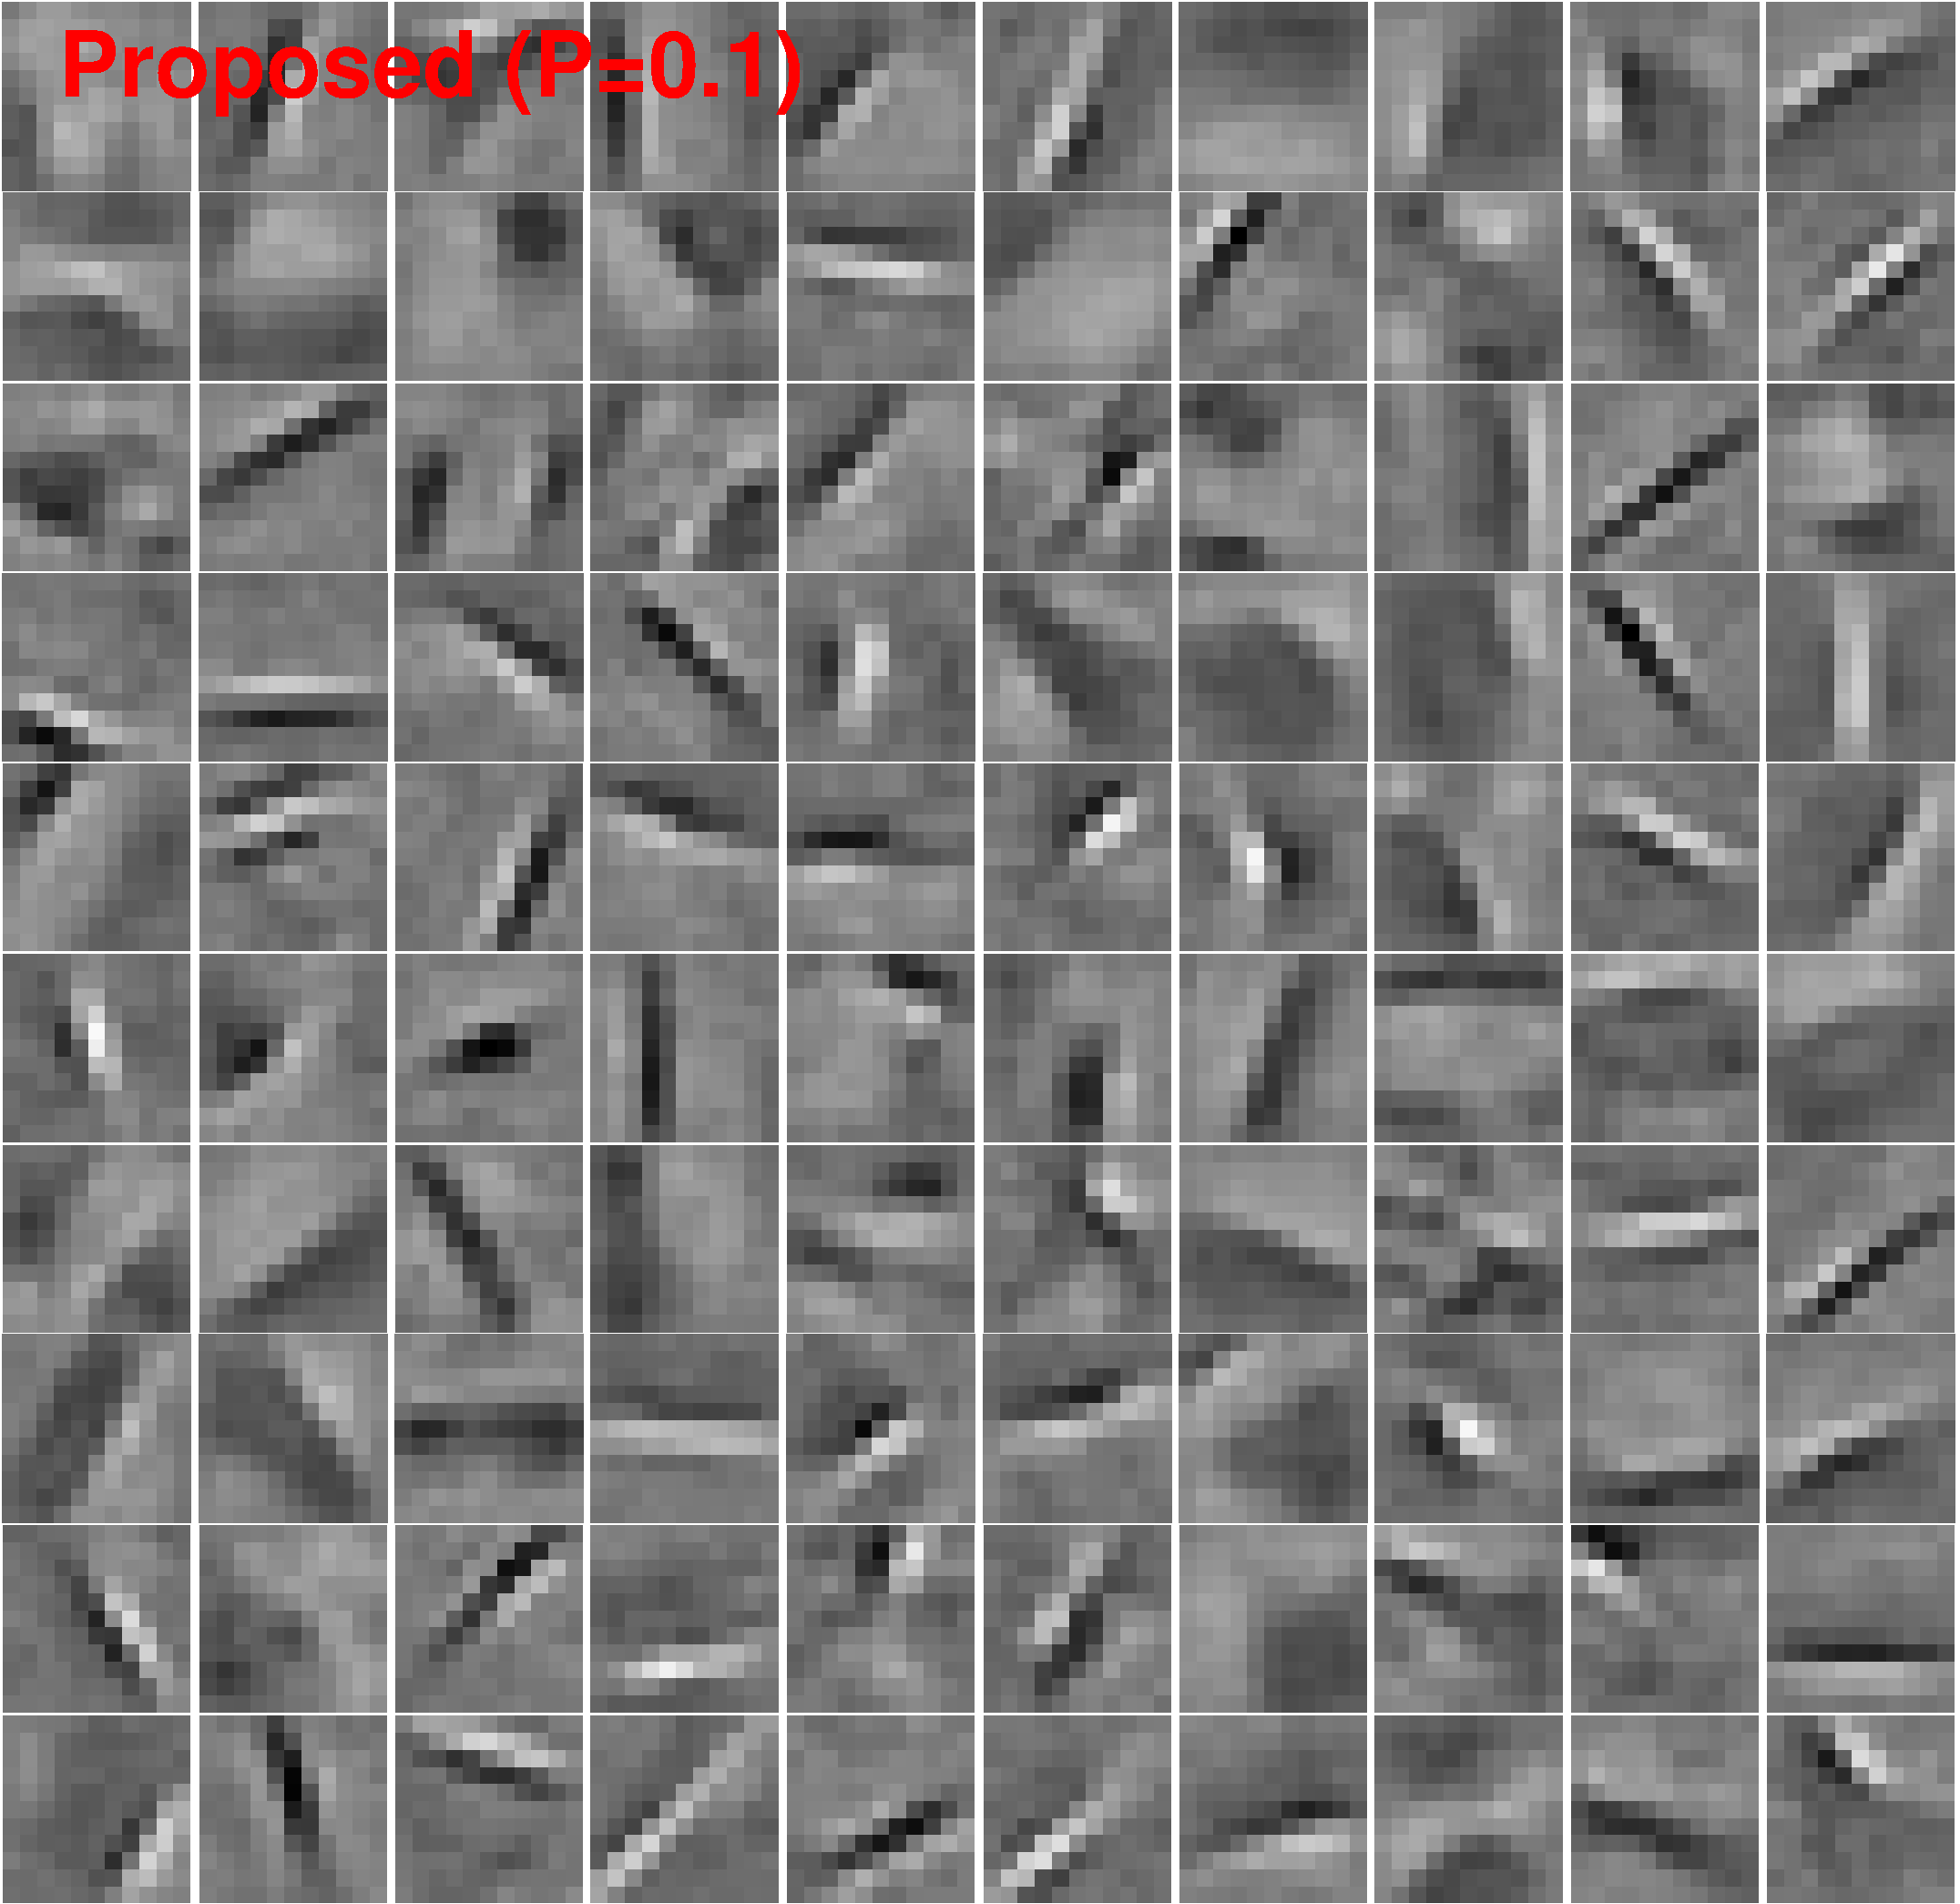
\includegraphics[width=1\linewidth]{figure/batchFruit100.pdf}
  \vspace{0.1cm}
\end{subfigure}
\begin{subfigure}{0.49\textwidth}
  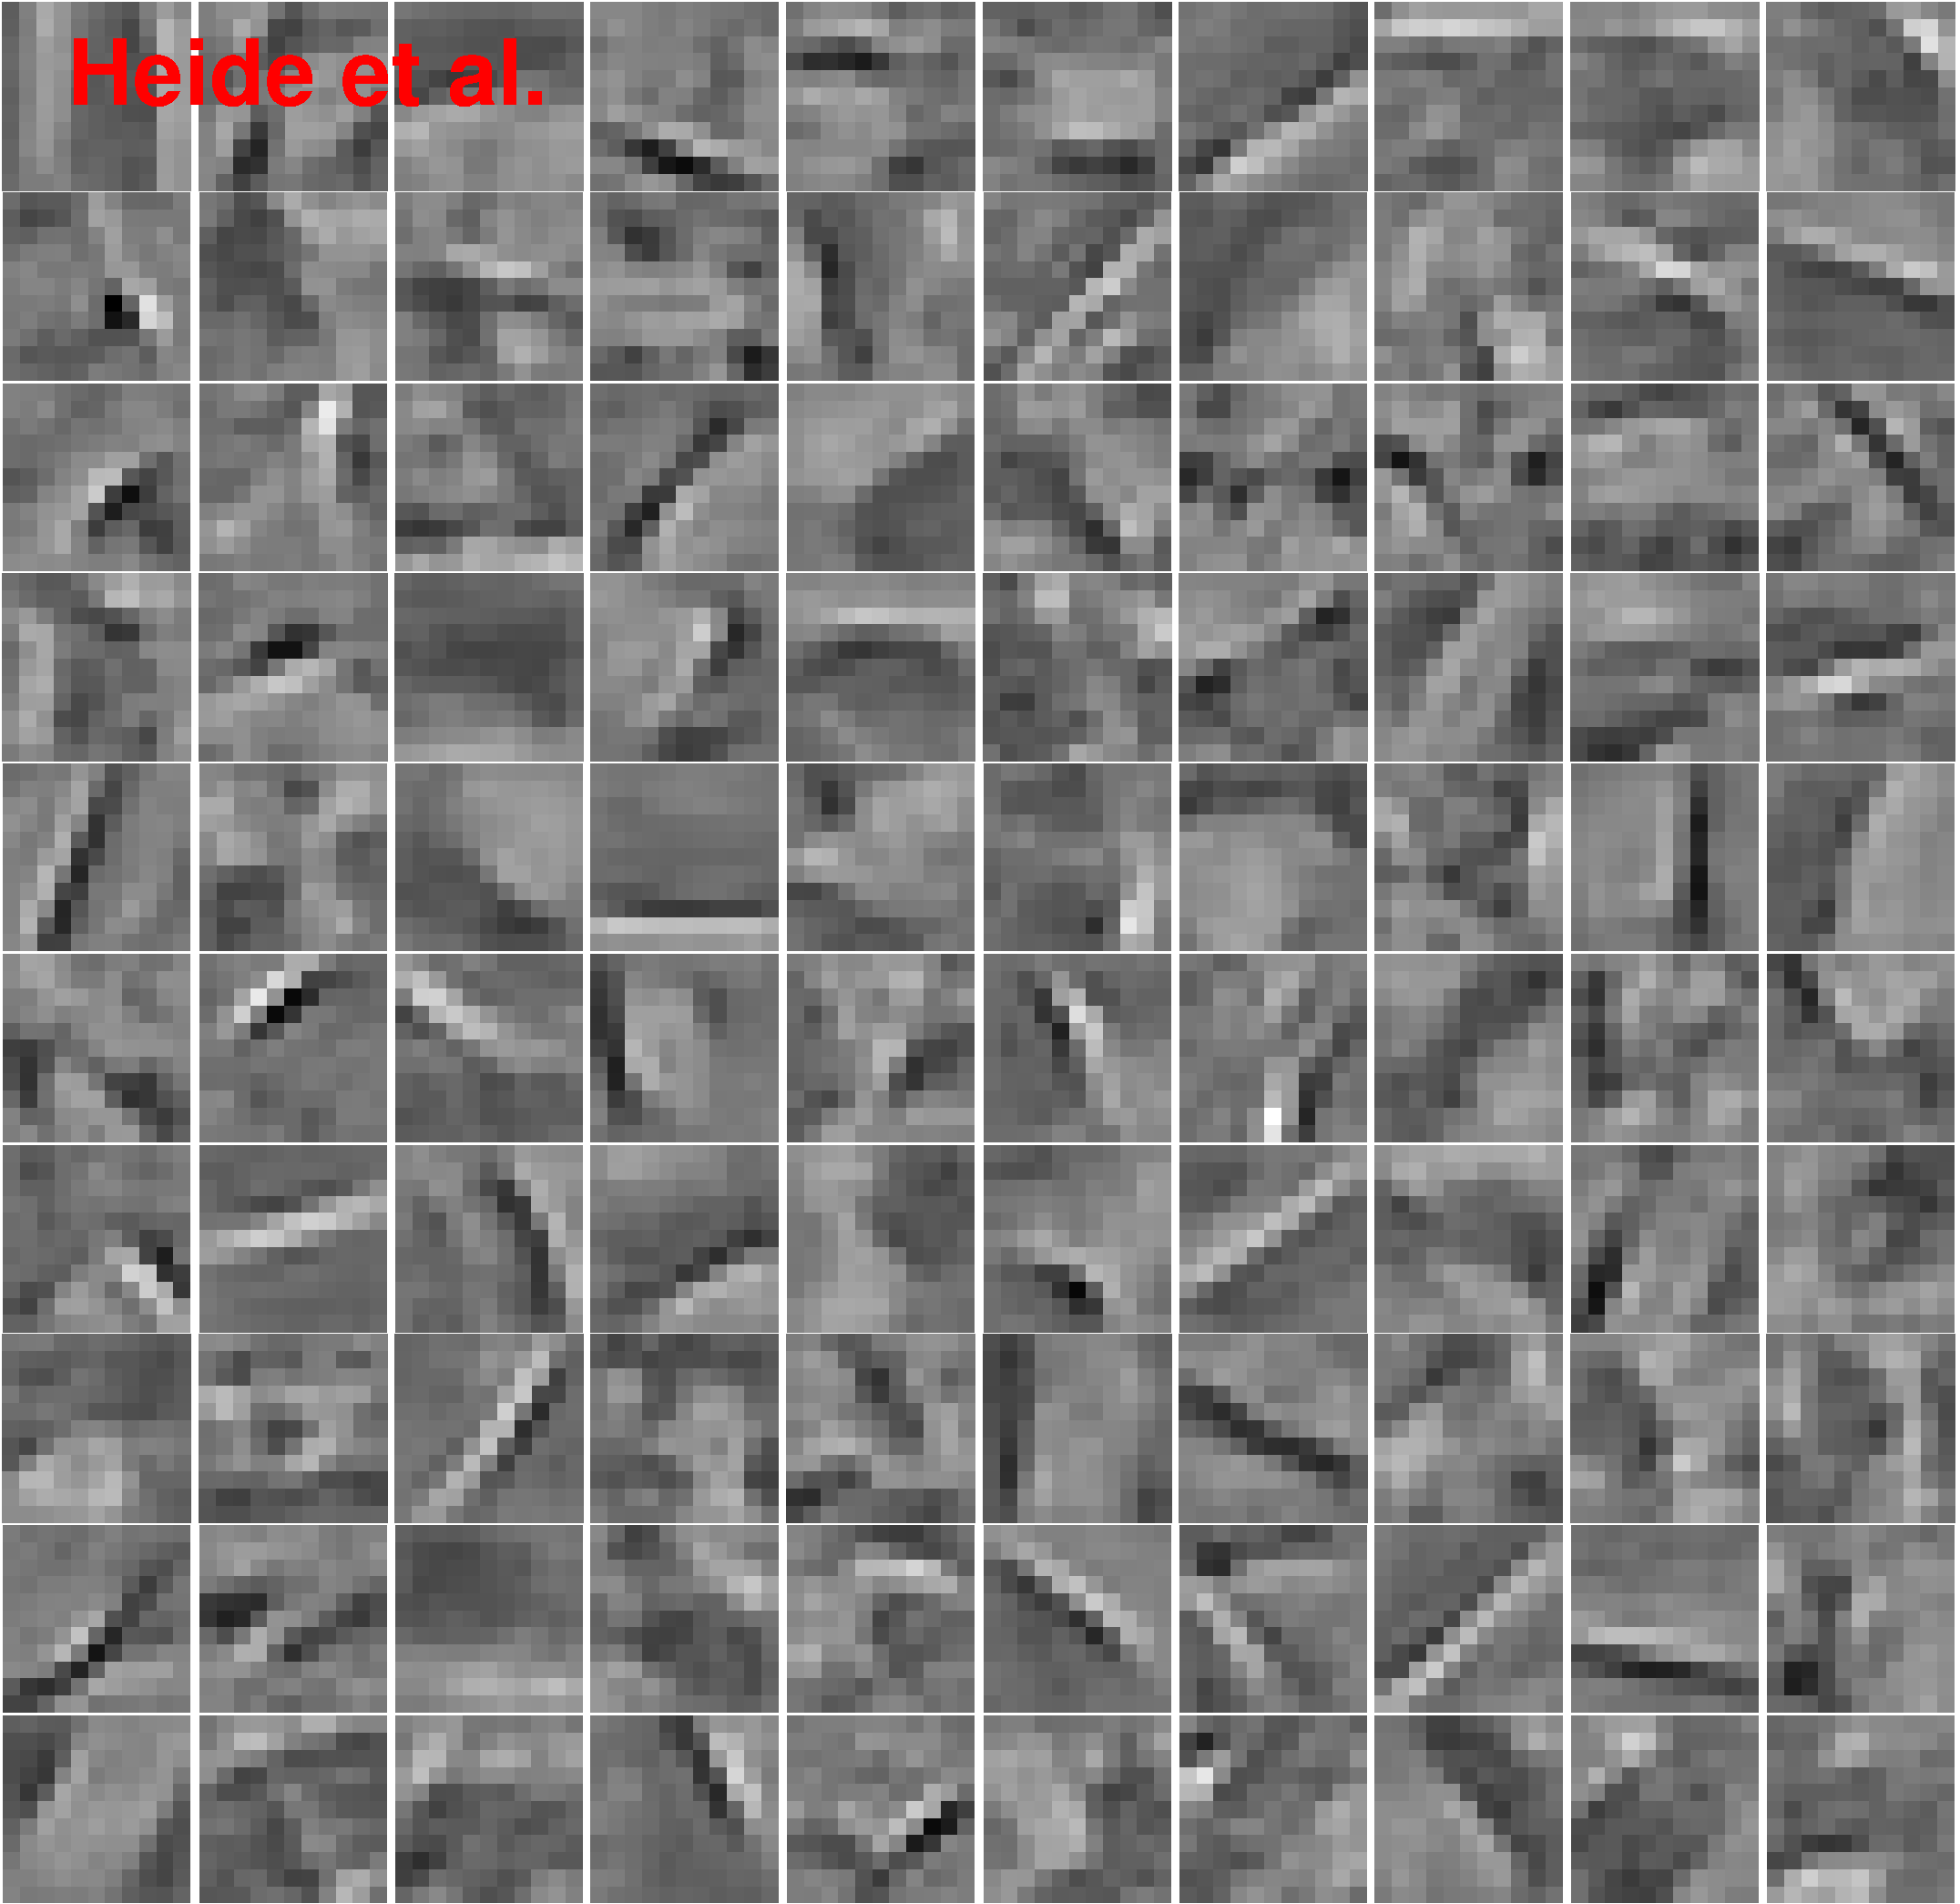
\includegraphics[width=1\linewidth]{figure/heideFruit100.pdf}
  \end{subfigure}
\caption{Zoom-in view of the filters from Figure~\ref{fig:subsampleResult}.}
\end{figure}


\section{Additional Experiments}
In order to show the robustness of the proposed algorithms, We also conduct experiments on city dataset. We first compare SBCSC with the state-of-the-art batch-mode algorithm~\cite{heide2015fast}, and the results are shown in Fig.\ \ref{fig:subsampleResult-city}. Similar to the results shown in Fig.\ \ref{fig:subsampleResult}, SBCSC, with $p=0.1$, outperforms the compared batch-mode algorithm with better outcomes and runtime performance. Since the learning is performed on handful datasets, both of them learn quite a few data-specific image features. The reconstruction quality also shows a shortage of the generalization ability. For example, the eighth image, which contains a large portion of texture information existed in the filters learned from city dataset, can be significantly better reconstructed by such filters compared to those learned from fruit dataset, while it may have poorer performance on other types of images. Furthermore, compared with the over-complete dictionary, we can observe that the presented over-complete dictionary contains both of the image features (superficially similar) appeared in the filters learned from fruit and city dataset, even though they use totally different training images. It also experimentally shows a better reconstruction performance on all kinds of testing images.

\begin{figure}[h]
\centering
\begin{subfigure}{0.5\textwidth}
  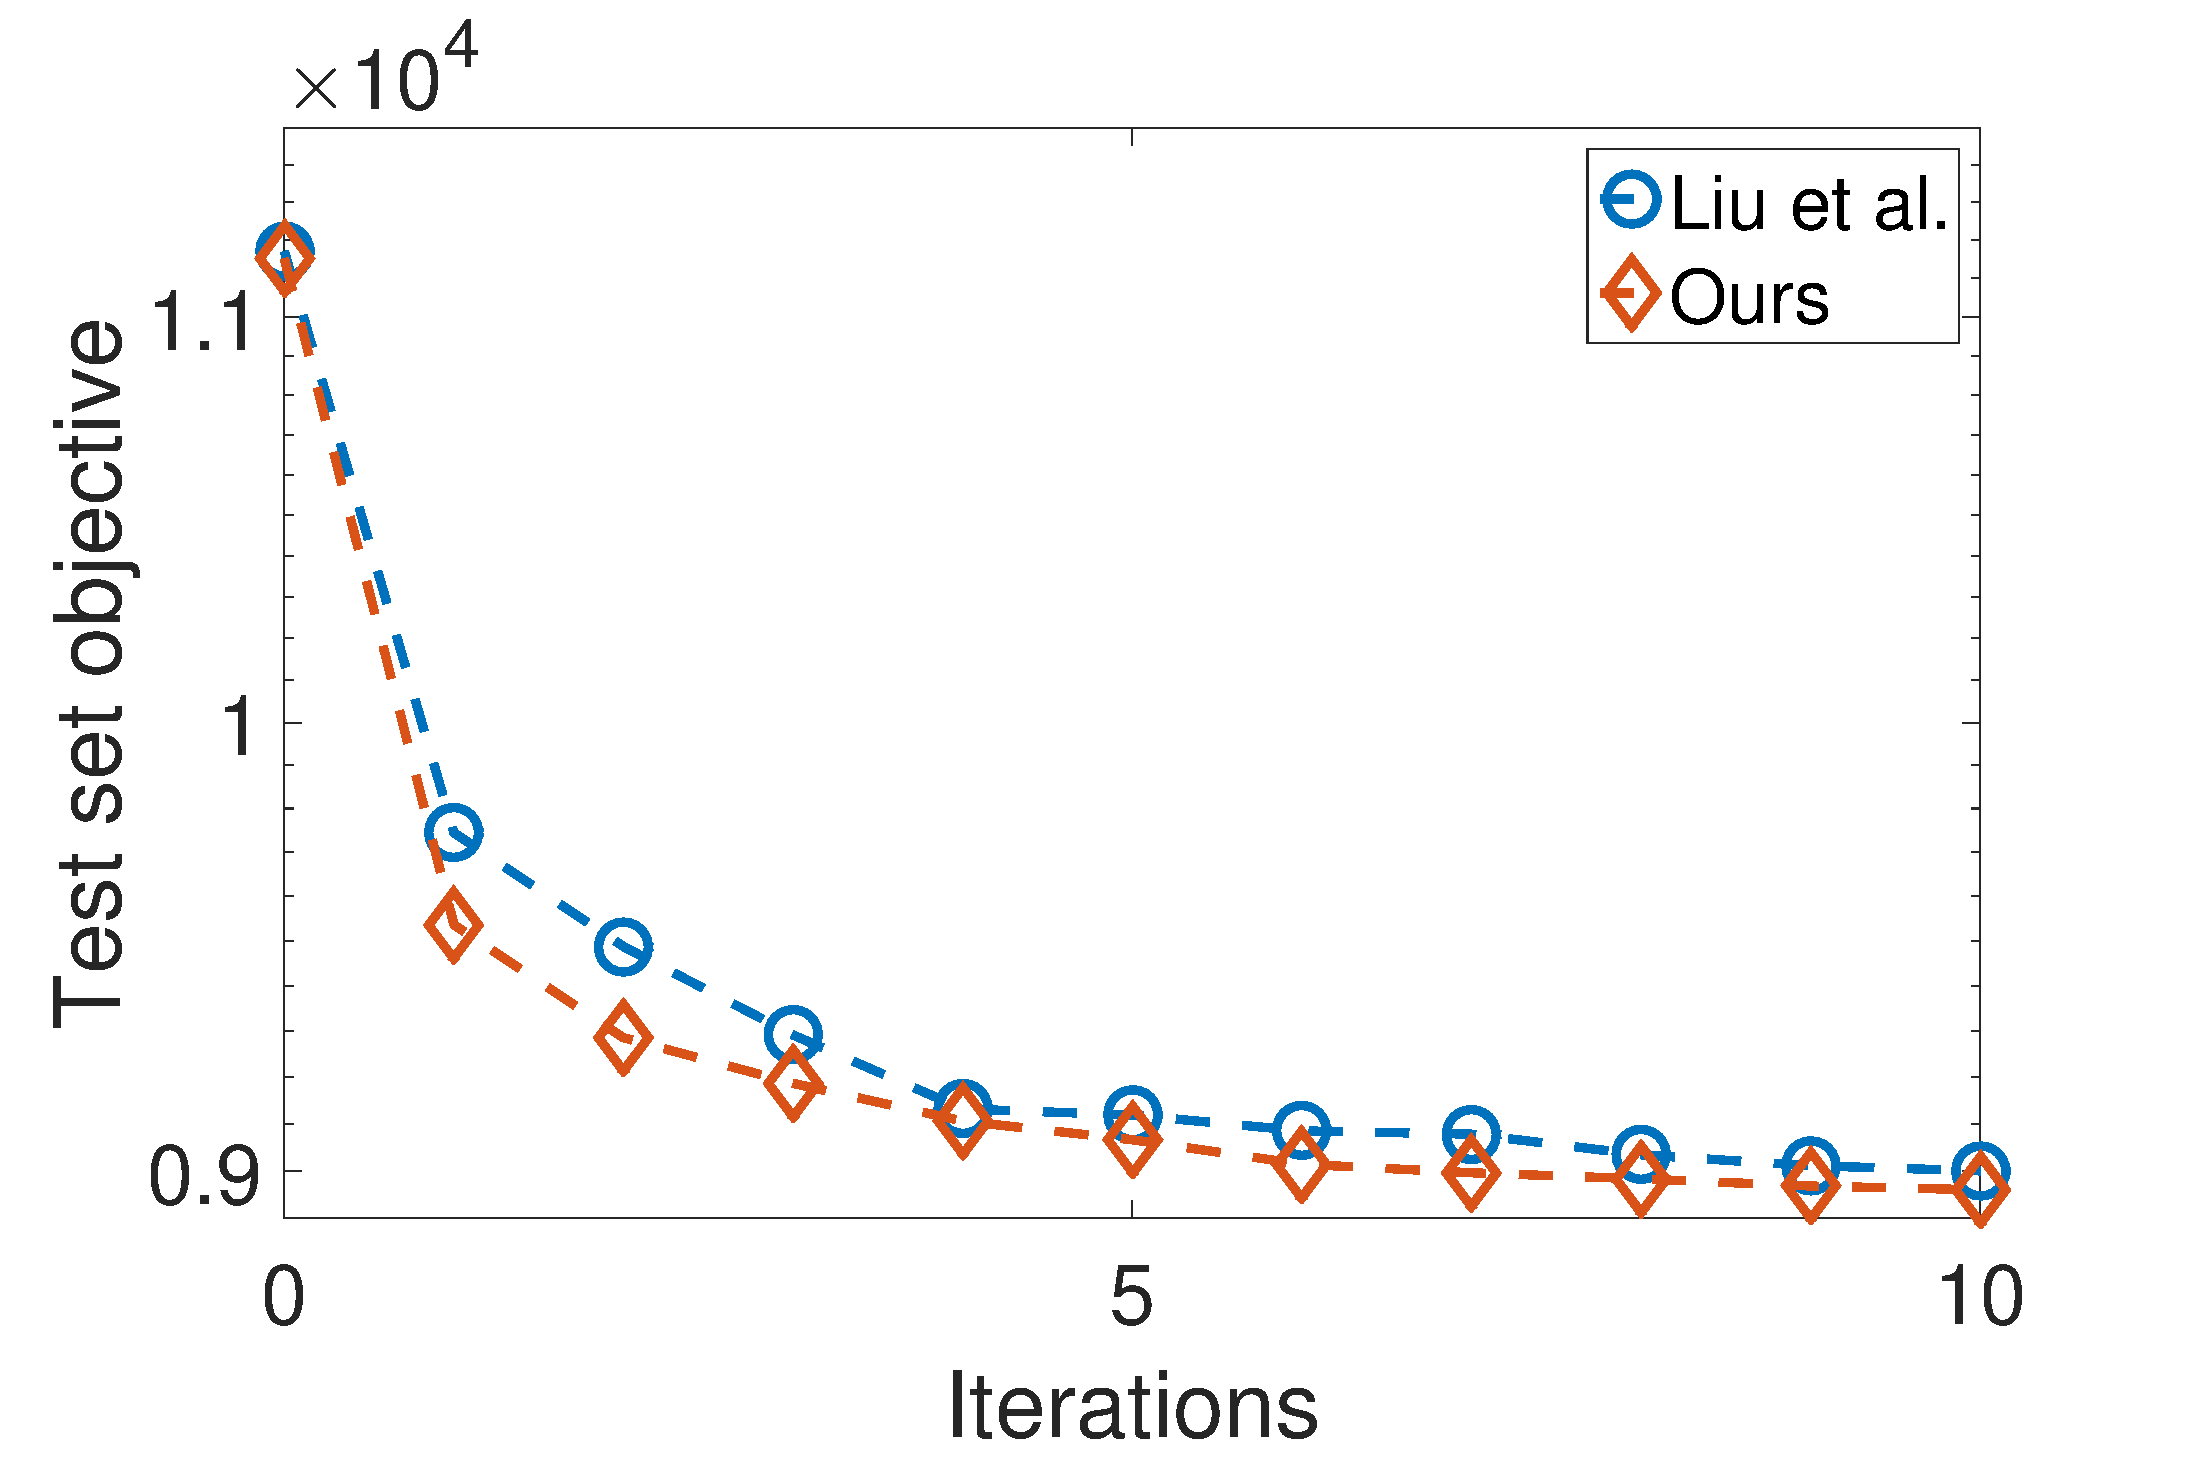
\includegraphics[width=1\linewidth]{figure/onlineVSliu-ite.pdf}
\end{subfigure}
\begin{subfigure}{0.5\textwidth}
  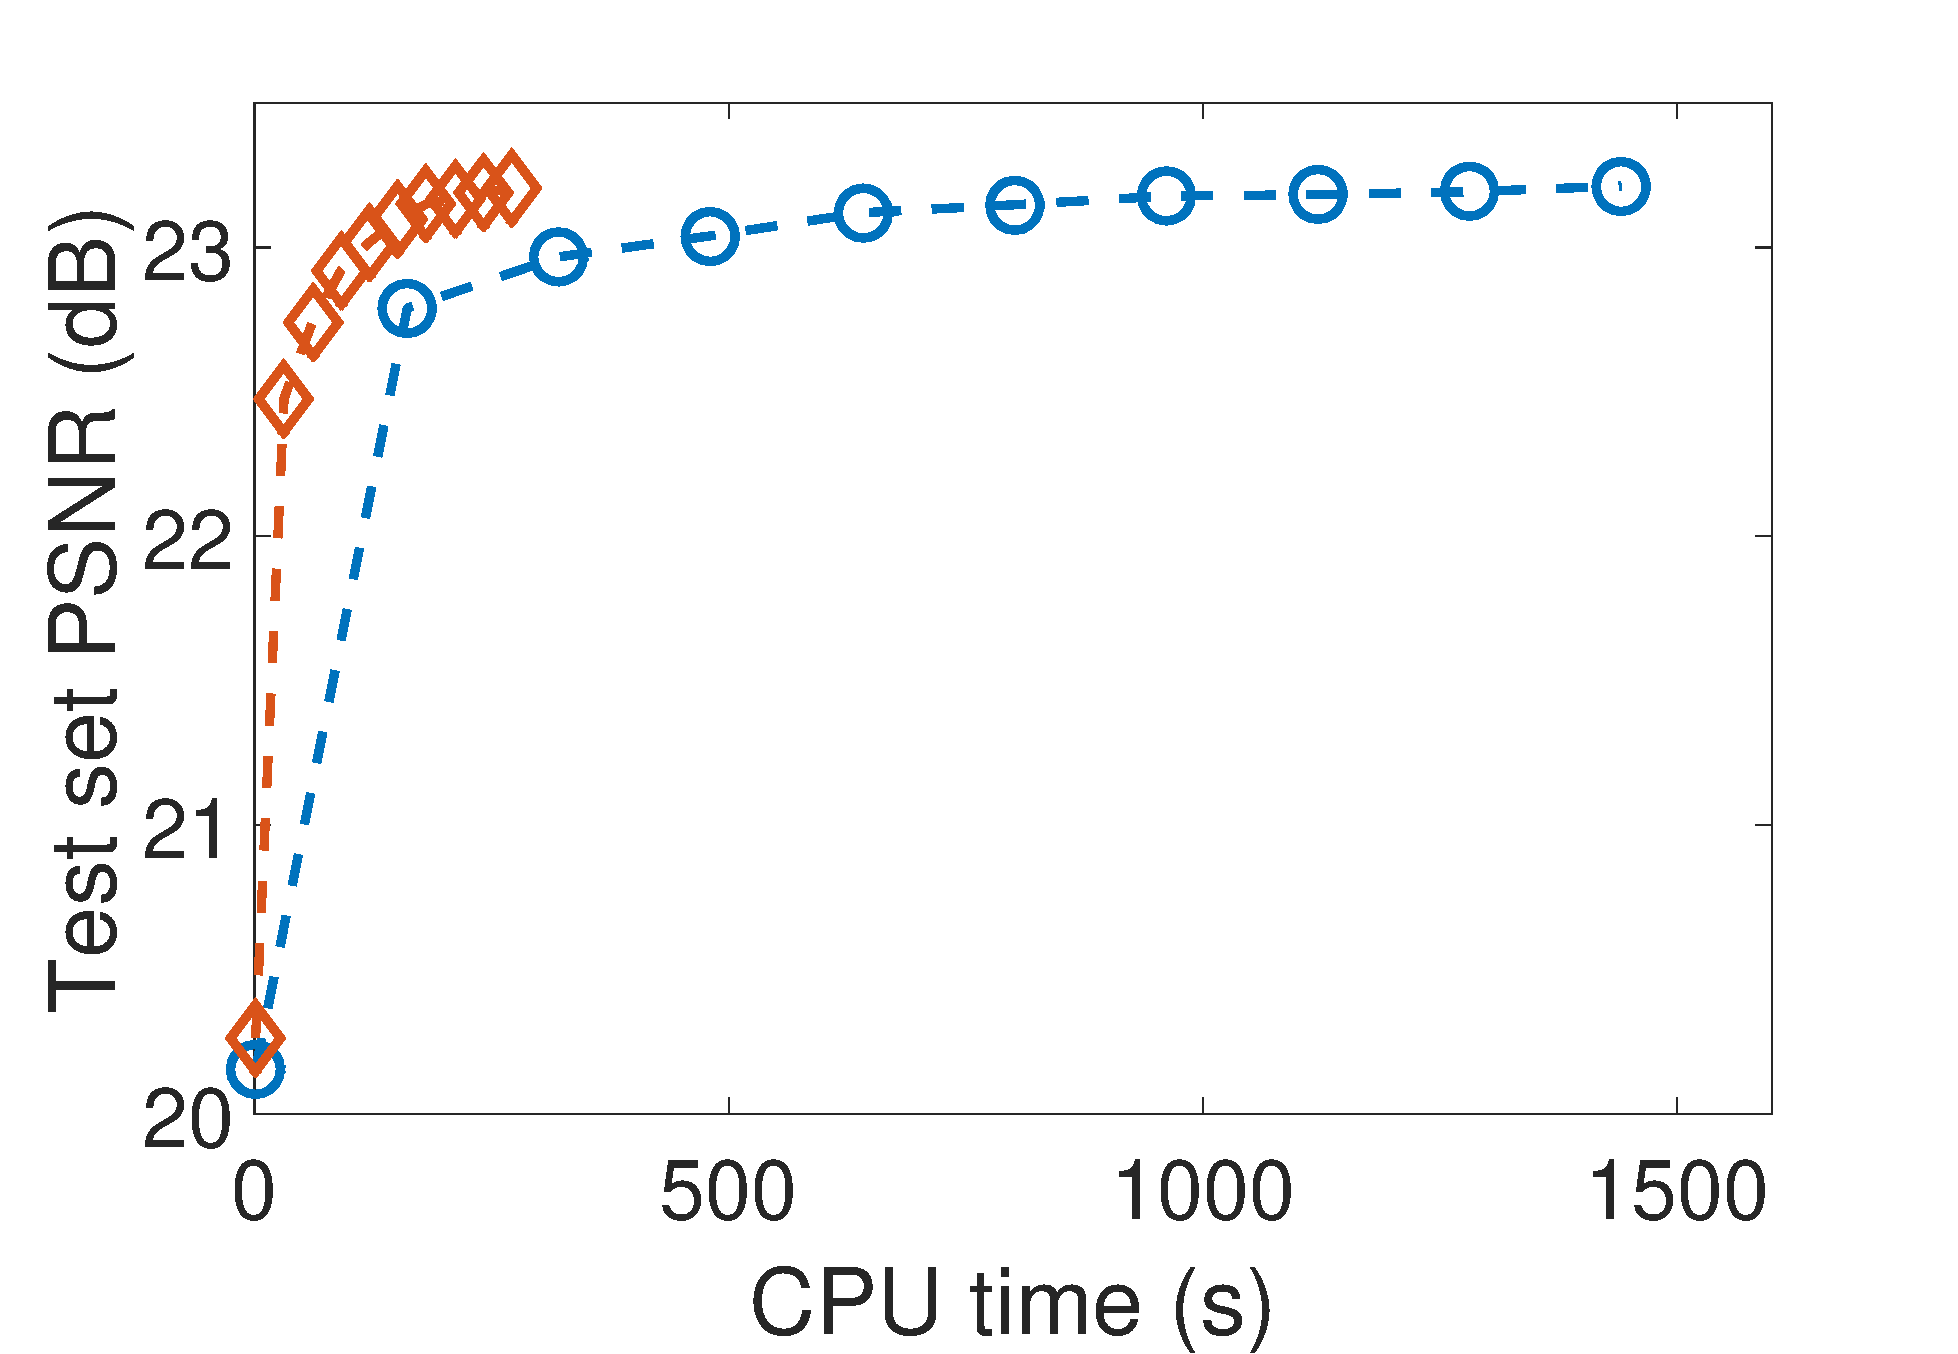
\includegraphics[width=1\linewidth]{figure/onlineVSliu-time.pdf}
\end{subfigure}

\caption{Experimental results obtained on city dataset. Top: Convergence of the test set objectives for our method (SOCSC) and the state-of-the-art online approach~\cite{liu-2018-first}. Bottom: Testing PSNR with respect to execution time.}
\label{fig:onlineSmall-city}
\end{figure}

\begin{figure*}[h]
\begin{subfigure}{0.5\textwidth}
  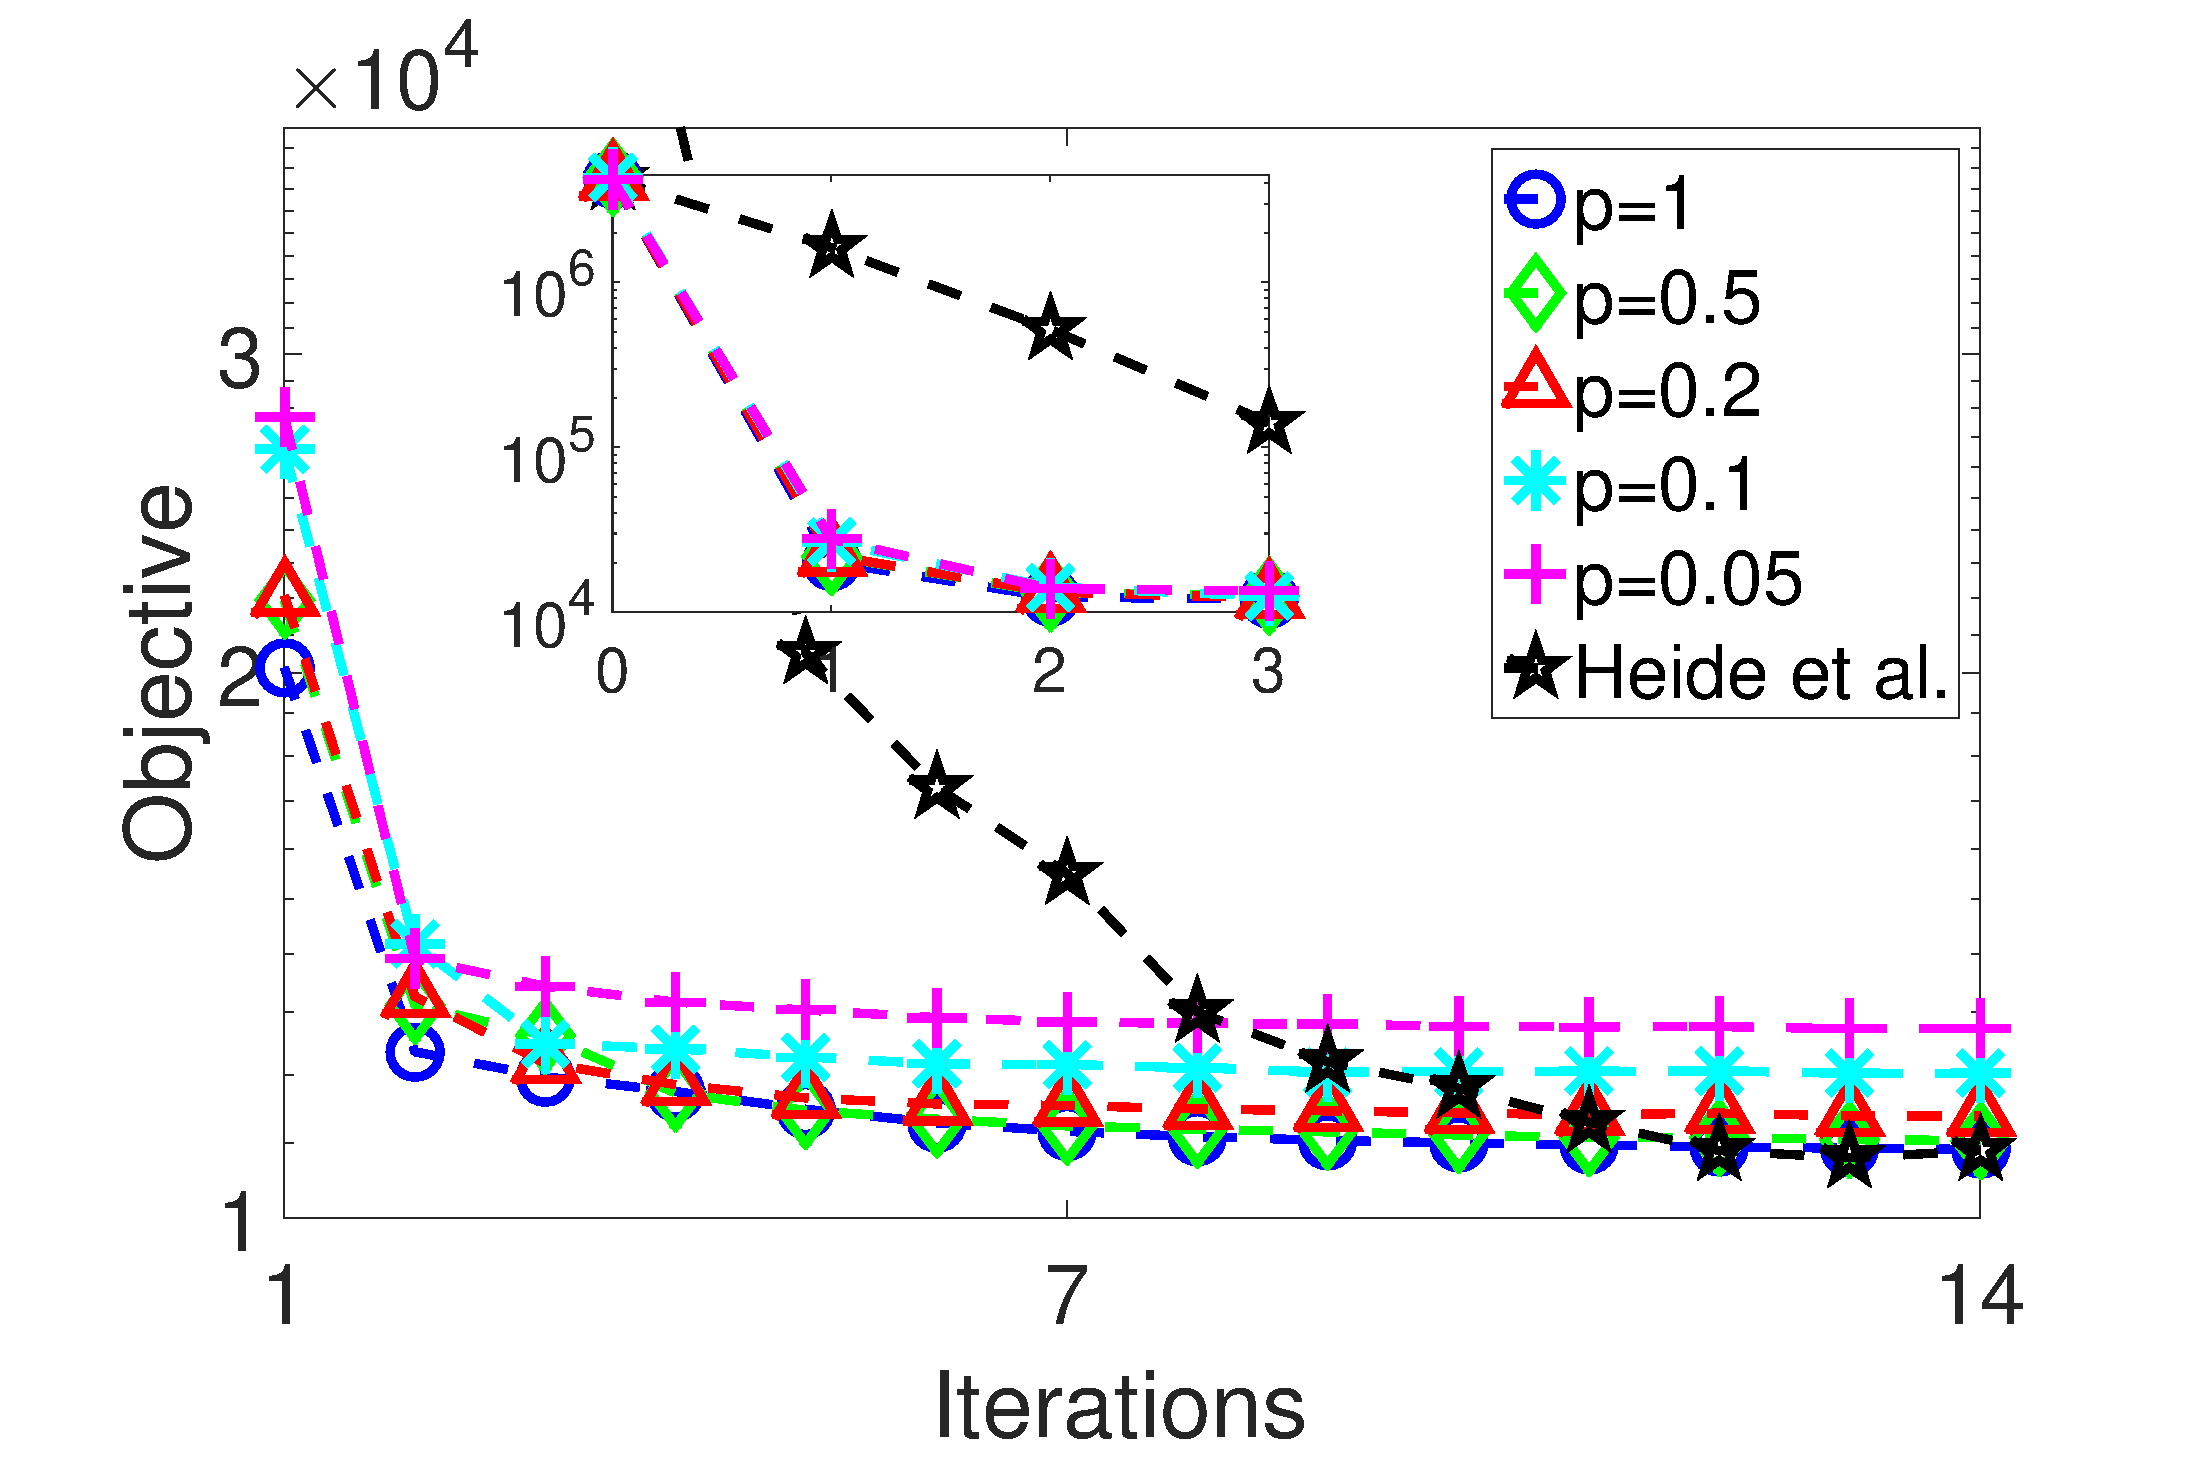
\includegraphics[width=1\linewidth]{figure/iteVSobj-city.pdf}
\end{subfigure}
\begin{subfigure}{0.5\textwidth}
  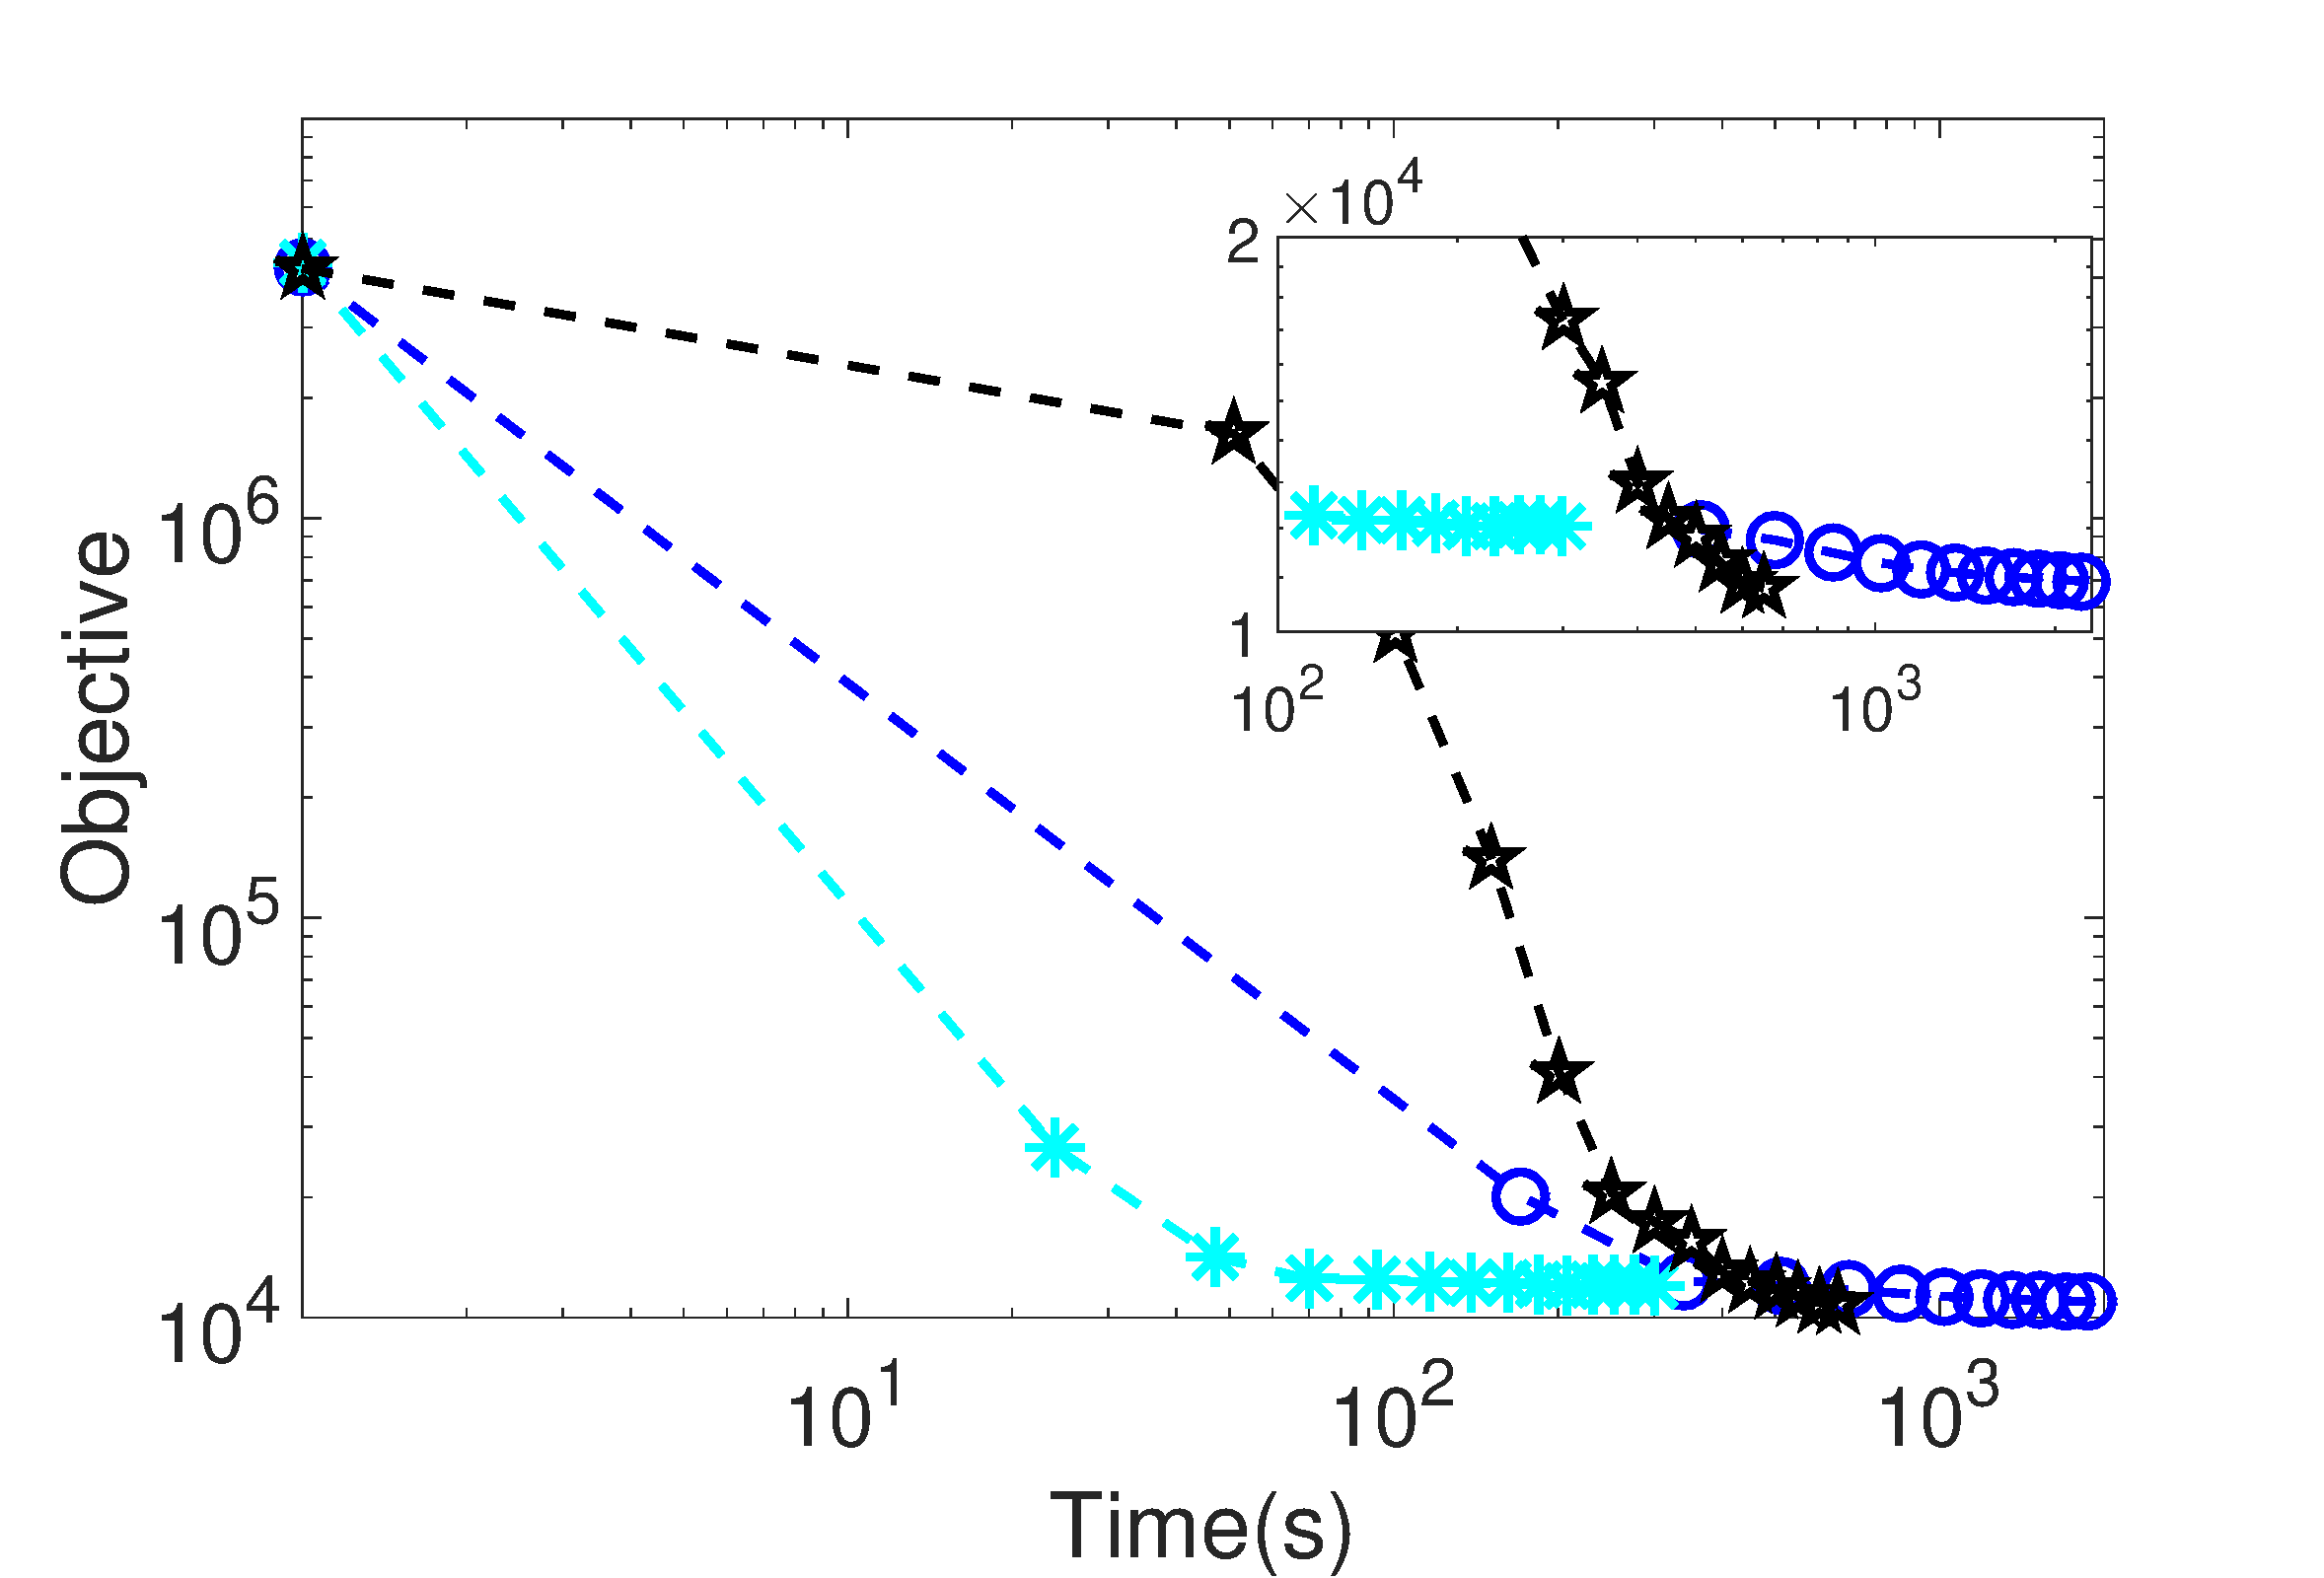
\includegraphics[width=1\linewidth]{figure/timeVSobj-city.pdf}
\end{subfigure}

\centering
\begin{subfigure}{0.49\textwidth}
  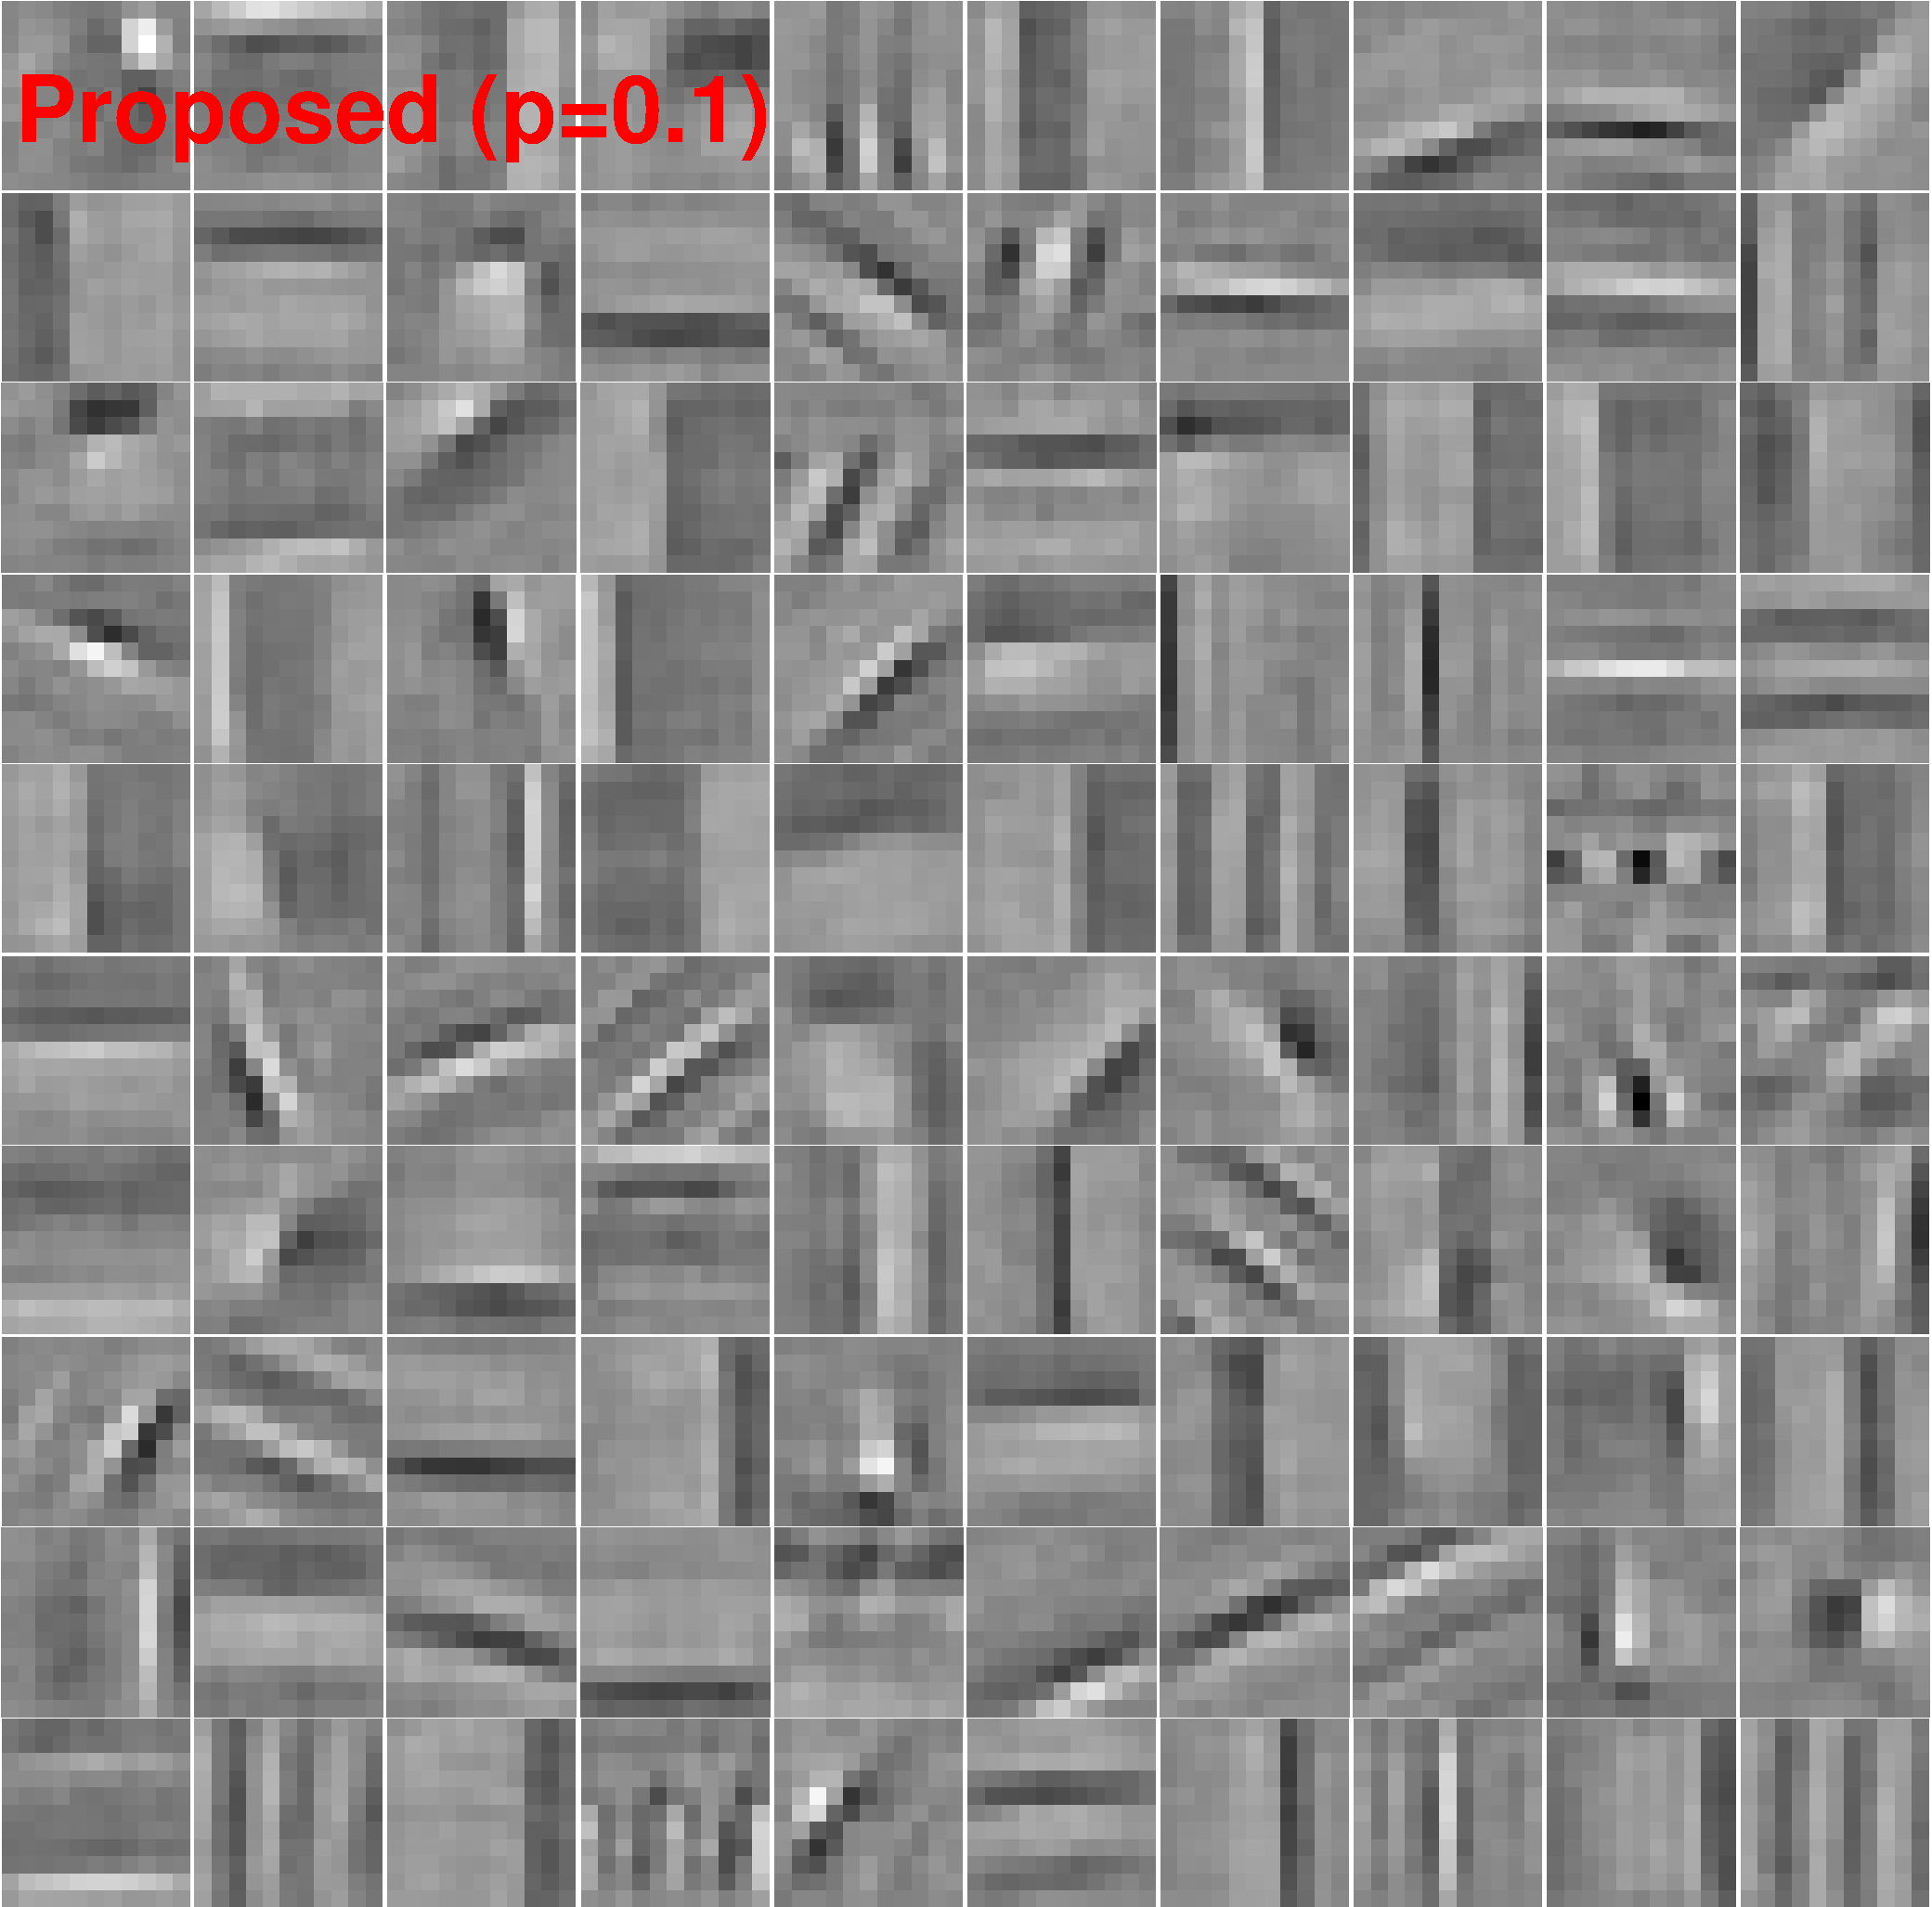
\includegraphics[width=1\linewidth]{figure/batchCity100.pdf}
\end{subfigure}
\begin{subfigure}{0.49\textwidth}
  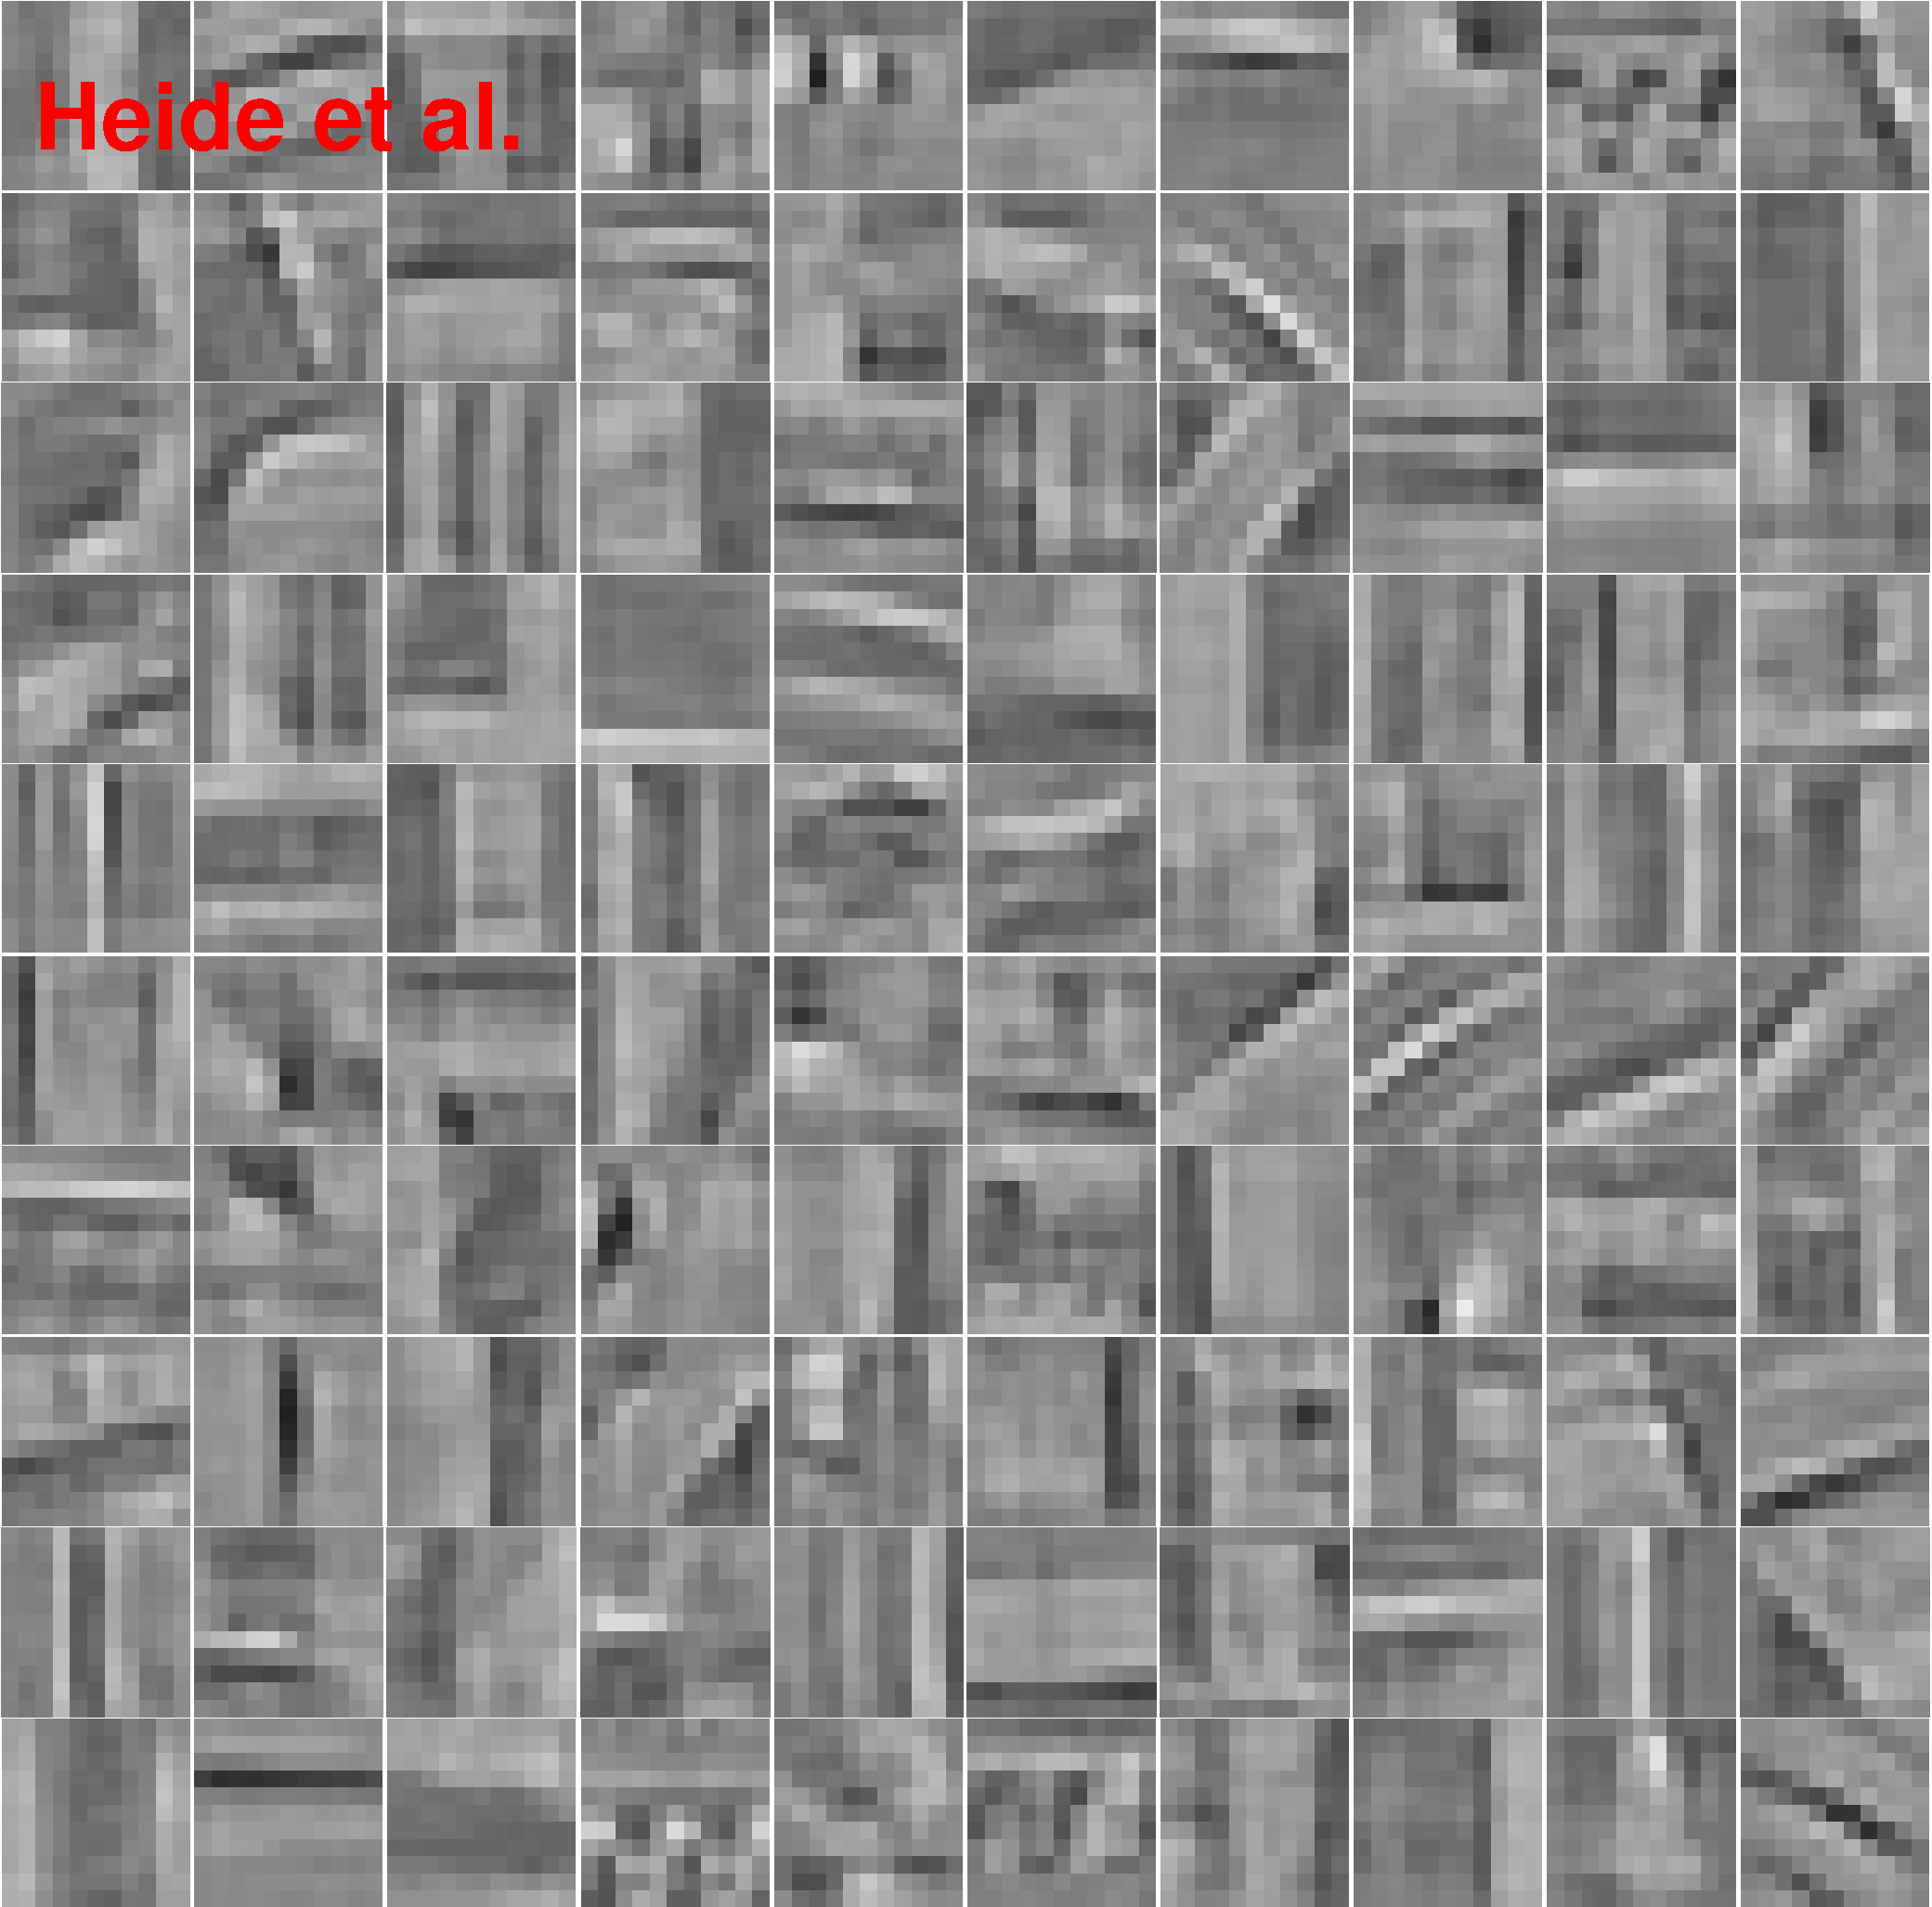
\includegraphics[width=1\linewidth]{figure/heideCity100.pdf}
\end{subfigure}
\vspace{0.2cm}

    \resizebox{0.8\linewidth}{!}{
        \begin{tabular}{|c||c|c|c|c|c|c|c|c|c|c|}
            \cline{1-11}
            Image & 1 & 2 & 3 & 4 & 5 & 6 & 7 & 8 & 9 & 10 \\
            \hline
            PSNR~\cite{heide2015fast} & 29.67 & \textbf{28.14} & 29.58 & 29.69 & 28.74 & 29.43 & 27.89  & 30.13 & 27.03 & 30.61 \\
            \hline
            PSNR ours & \textbf{29.78} & \textbf{28.14} & \textbf{29.67}  & \textbf{29.85} & \textbf{28.88} & \textbf{29.95} & \textbf{27.97} & \textbf{30.37} & \textbf{27.14} & \textbf{30.89} \\
            \hline
        \end{tabular} }

\caption{Experimental results obtained on the city dataset. Top: Convergence comparison between the-state-of-art batch method~\cite{heide2015fast} and SBCSC with different subsampling probability. Middle: Learned filters by SBCSC with $p=0.1$ and the comparable method. Even though these dictionaries look similar, our method learns more smooth filters. Compared to the learned filters in Fig.\ \ref{fig:subsampleResult}, they have different representations of the dictionaries, where data-specific features are learned from handful training images. Bottom: Numerical comparisons of the reconstruction quality obtained by the presented filters.}
\label{fig:subsampleResult-city}
\end{figure*}

We then compare SOCSC with the state-of-the-art online algorithm~\cite{liu-2018-first} on city dataset, the results of which are shown in Fig.\ \ref{fig:onlineSmall-city}. Similar to the results presented in Fig.\ \ref{fig:onlineSmall}, our method obtains comparable outcomes, meanwhile, achieves roughly $6 \times$ speedup.

\section{Over-complete Dictionary and Large Datasets}
In this section, we verify the importance of a large dataset when learning the over-complete dictionary. in Fig.~\ref{fig:overCompleteDic-dataset}, we show a visual and quantitative comparisons between the over-complete dictionaries respectively learned by batch-mode algorithm on small dataset (the fruit dataset) and online-mode algorithm on large dataset (1000 images). Most of the filters learned from small dataset have poor structures and reveal very limited representative ability. The numerical results also demonstrate that it even shows a degraded reconstruction performance compared to the under-complete dictionary. Owing to plentiful training samples, our over-complete dictionary not only shows visually decent structures and more representative image features, but also leads to a significant improvement on image reconstruction. Based on all experimental results, it implies that the number of filters and number of training samples are both essential in the CSC model, therefore, the proposed algorithm has prominent advantages over the existing approaches.

\begin{figure*}[h]
\centering
  \begin{subfigure}{0.5\textwidth}
  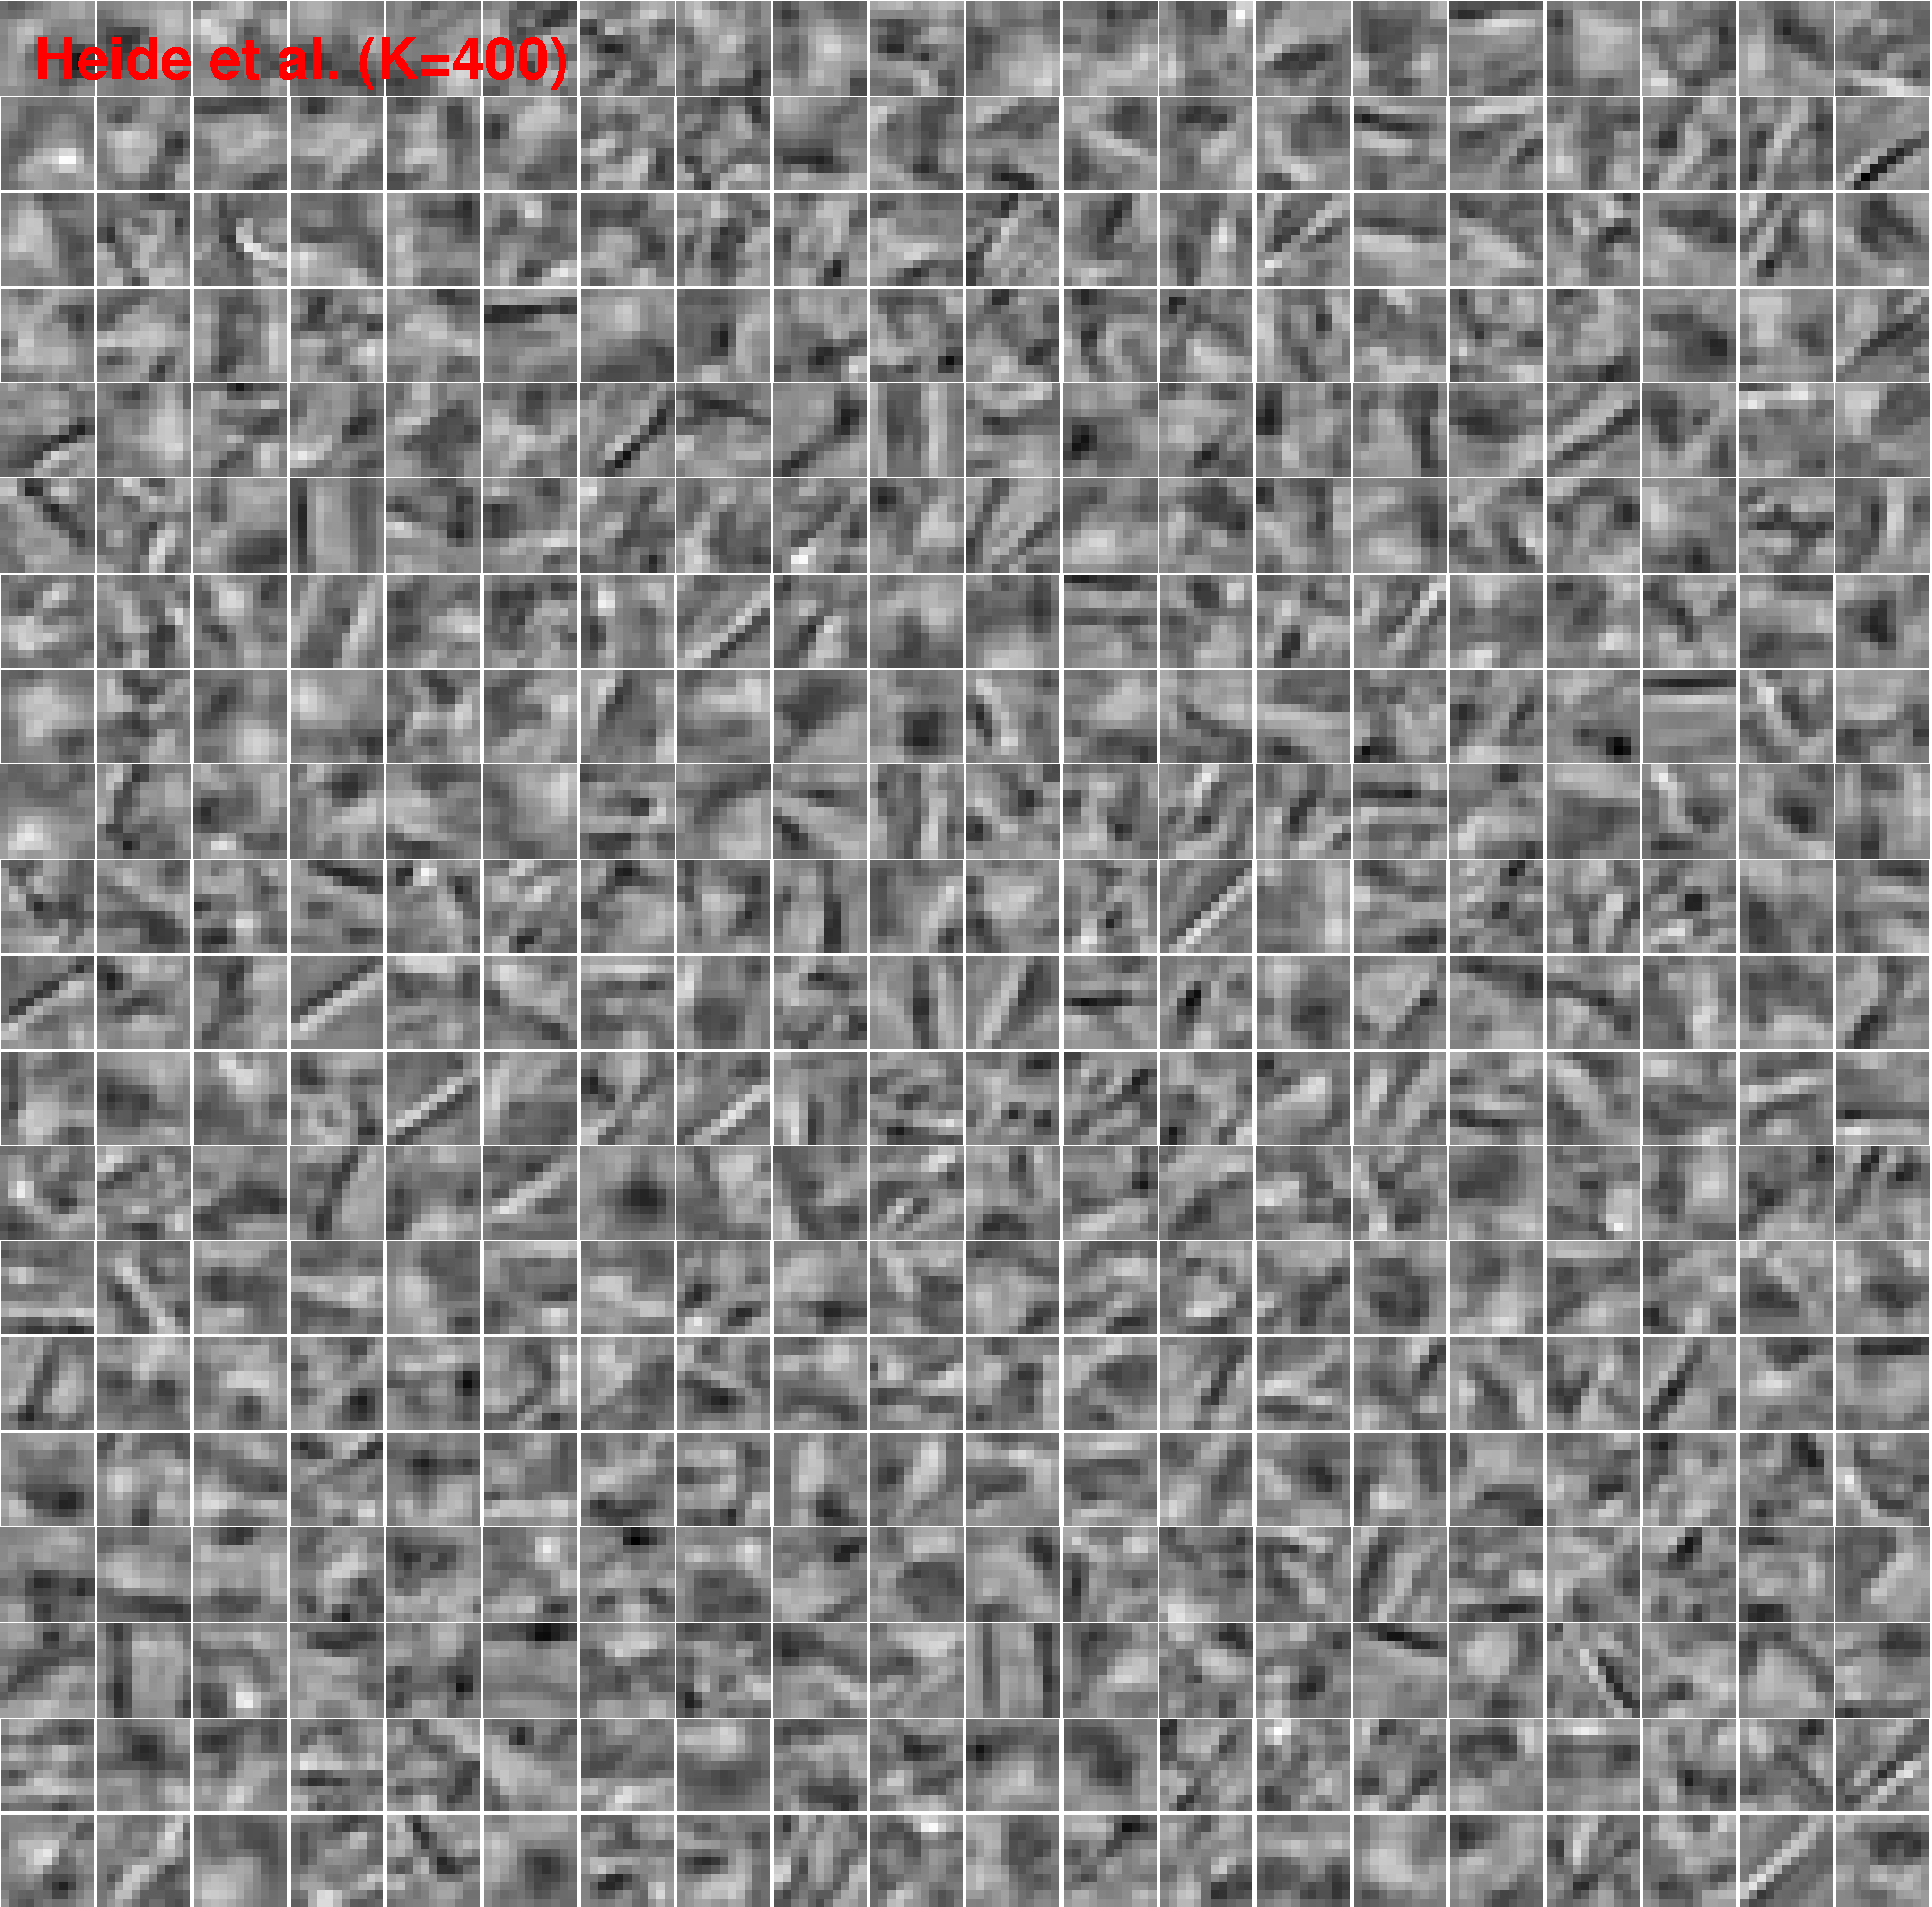
\includegraphics[width=1\linewidth]{figure/heide400-supple.pdf}
  \end{subfigure}
  \vspace{0.2cm}
  \begin{subfigure}{0.5\textwidth}
  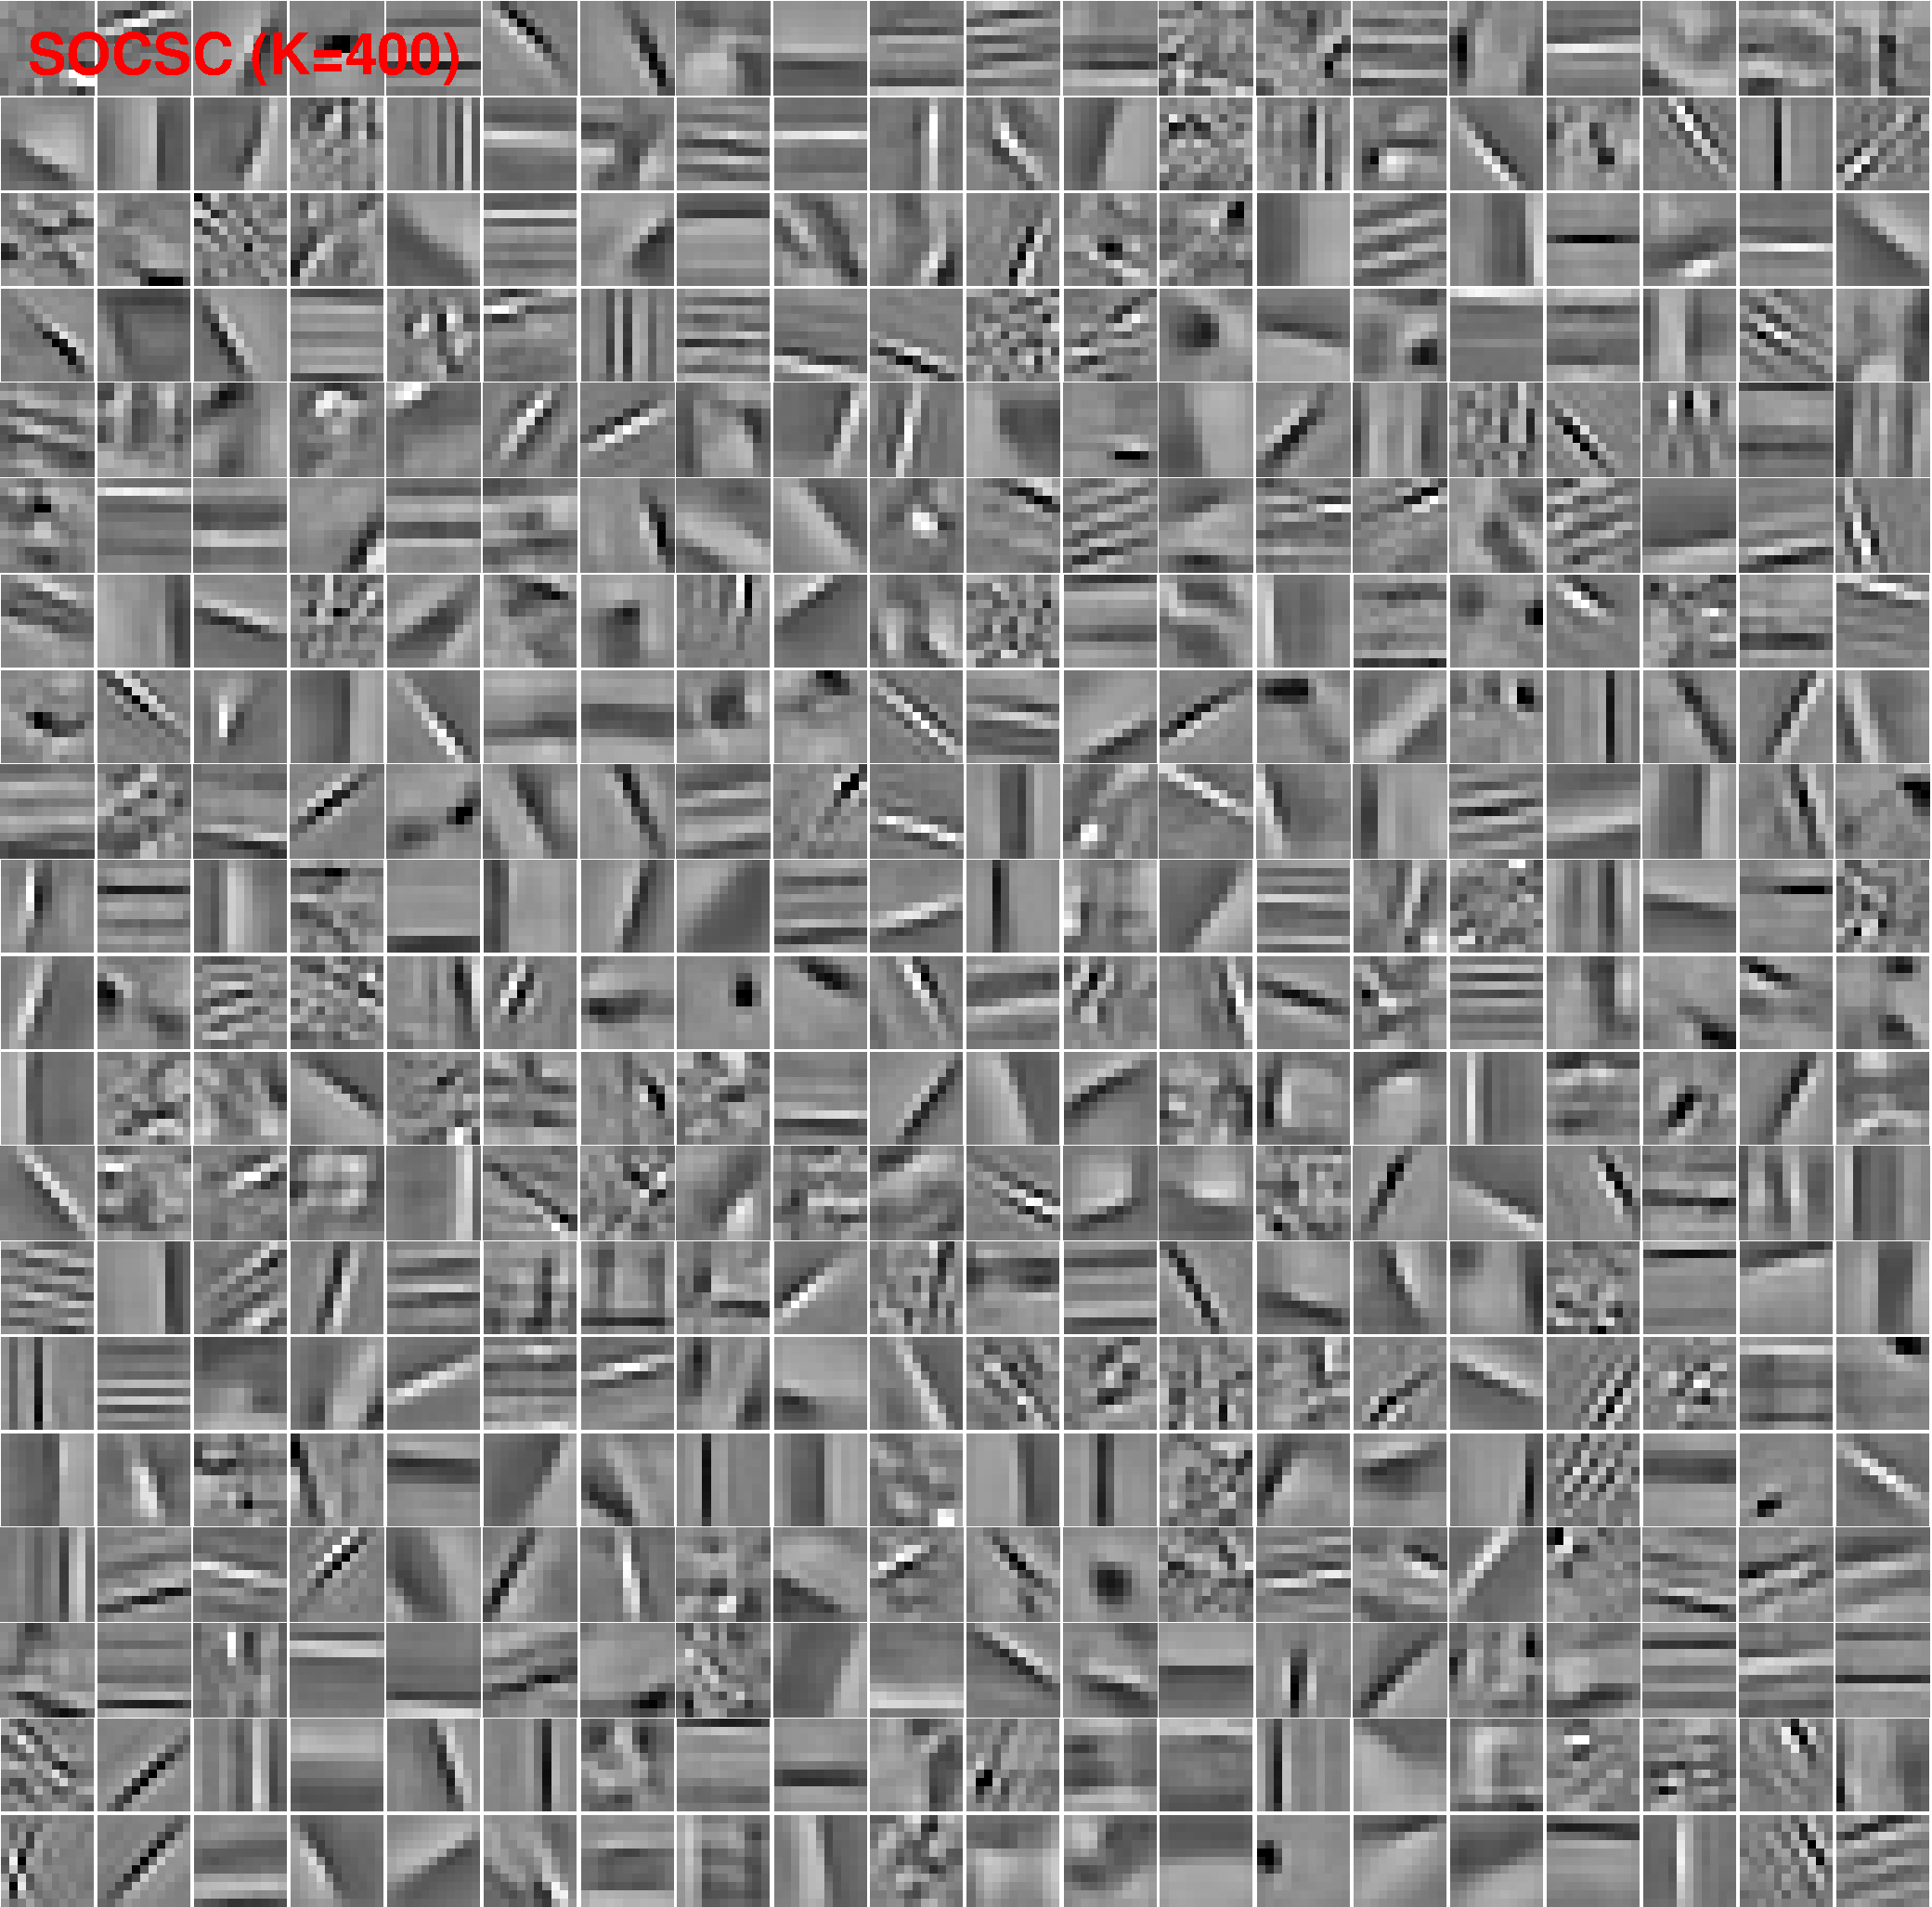
\includegraphics[width=1\linewidth]{figure/online400-supple.pdf}
  \end{subfigure}
  \vspace{0.2cm}

    \resizebox{0.8\linewidth}{!}{
        \begin{tabular}{|c||c|c|c|c|c|c|c|c|c|c|}
            \cline{1-11}
            Image & 1 & 2 & 3 & 4 & 5 & 6 & 7 & 8 & 9 & 10 \\
            \hline
            PSNR~\cite{heide2015fast} & 29.60 & 28.11 & 29.47 & 28.98 & 28.79 & 29.21 & 28.03  & 29.31 & 27.42 & 30.52 \\
            \hline
            PSNR ours & \textbf{30.24} & \textbf{28.34} & \textbf{29.95}  & \textbf{30.30} & \textbf{29.43} & \textbf{29.96} & \textbf{28.24} & \textbf{30.57} & \textbf{27.72} & \textbf{31.67} \\
            \hline
        \end{tabular} }
  \caption{ Visual and numerical comparisons between the learned over-complete dictionaries by batch-mode algorithm and by online-mode algorithm. Top: Over-complete dictionary learned by batch CSC model~\cite{heide2015fast} on small dataset, and proposed online CSC model (SOCSC) on large dataset. Bottom: Respective reconstruction quality for these two over-complete dictionaries.}
  \label{fig:overCompleteDic-dataset}
\end{figure*} 